\documentclass[UTF8,a4paper,12pt]{ctexart}
\usepackage[margin=2.5cm]{geometry}
\usepackage{graphicx}
\usepackage{booktabs}
\usepackage{longtable}
\usepackage{tabularx}
\usepackage{array}
\usepackage{calc}
\usepackage{textcomp}
\usepackage{amsmath}
\usepackage{amssymb}
\usepackage{enumitem}
\usepackage{caption}
\usepackage{fancyhdr}
\usepackage{listings}
\usepackage{float}
\usepackage[hidelinks]{hyperref}
\usepackage{color}
\usepackage{tikz}
\usepackage{tikz-cd}

\usepackage{dirtree}
\usepackage{xcolor}

\usetikzlibrary{shapes.geometric, arrows.meta, positioning}

\setcounter{tocdepth}{3}
\setlength{\parindent}{2em}
\setlength{\parskip}{0.35em}
\setlist{itemsep=0.2em, topsep=0.3em, parsep=0pt, partopsep=0pt}
\renewcommand{\arraystretch}{1.2}
\graphicspath{{src/assets/}{assets/}}
\captionsetup{font=small,labelfont=bf,position=bottom}
\captionsetup[table]{position=top,skip=6pt}
\pagestyle{fancy}
\fancyhf{}
\fancyfoot[C]{\thepage}
\renewcommand{\headrulewidth}{0pt}
\renewcommand{\footrulewidth}{0pt}
\newcolumntype{L}[1]{>{\raggedright\arraybackslash}p{#1}}
\newcolumntype{C}[1]{>{\centering\arraybackslash}p{#1}}
\newenvironment{threelongtable}[1]{%
  \setlength\LTleft{\fill}%
  \setlength\LTright{\fill}%
  \renewcommand{\arraystretch}{1.2}%
  \scriptsize
  \begin{longtable}{#1}%
}{%
  \end{longtable}%
}
\lstdefinelanguage{SystemVerilog}{
  morekeywords={module,endmodule,input,output,wire,reg,assign,always,begin,end,if,else,casez,default},
  sensitive=true,
  morecomment=[l]{//},
  morecomment=[s]{/*}{*/},
  morestring=[b]"
}
\lstdefinestyle{svcode}{
  language=SystemVerilog,
  basicstyle=\ttfamily\scriptsize,
  keywordstyle=\bfseries\color{blue},
  commentstyle=\color{gray},
  numbers=none,
  breaklines=true,
  columns=fullflexible,
  keepspaces=true,
  frame=tb,
  showstringspaces=false,
  captionpos=b,
  aboveskip=0.8em,
  belowskip=0.8em
}
\lstset{basicstyle=\ttfamily\small,breaklines=true,columns=fullflexible,frame=single}
\newcommand{\coverfield}[2]{%
  {\zihao{4}%\heiti
   \noindent\makebox[6em][l]{\heiti#1：}%
   \underline{\makebox[\dimexpr\textwidth-6em\relax][l]{\strut\heiti #2}}\par}%
}
\title{基于RISC-V指令集的CPU设计\\竞业达设计报告}
\author{队伍编号：CICC1004252\\团队名称：和溢位}
\date{}
\begin{document}
\begin{titlepage}
  \centering
  
\includegraphics[width=0.35\textwidth]{image1.png}\par\vspace{1.2cm}
  {\zihao{2}\bfseries 第十届\\全国大学生集成电路创新创业大赛\par}
  \vspace*{\fill}
  \begin{minipage}{\textwidth}
    \raggedright
    \setlength{\parindent}{0pt}
    \coverfield{报告类型}{设计报告}
    \vspace{0.45cm}
    \coverfield{参赛杯赛}{``竞业达"企业命题}
    \vspace{0.45cm}
    \coverfield{作品名称}{基于RISC-V指令集的CPU设计}
    \vspace{0.45cm}
    \coverfield{队伍编号}{CICC1004252}
    \vspace{0.45cm}
    \coverfield{团队名称}{和溢位}
		\vspace{2cm}
  \end{minipage}
\end{titlepage}
\tableofcontents
\clearpage

\begingroup
% \setlength{\parindent}{0pt}
\section*{快速预览简介}
\addcontentsline{toc}{section}{快速预览简介}

	 本项目设计并实现了一个基于 RV32I 指令集的 RISC-V CPU 内核，并完成了与竞业达 FPGA 外设的适配，
实现了赛题要求的 \textcolor{red}{\textbf{全部 37 条指令}}。

在 Vivado 2024 下完成综合与生成，时钟频率 \textcolor{red}{\textbf{250MHz 下 WNS 为正无违例}}，并在竞业达数字孪生平台上对 src0、src1、src2、test\_src 四组程序完成上板验证。
   三份性能测试运行时间分别为 8.7s、9.8s、10.6s，平均 CPI 为 1.61，对应 IPC 为 0.62。

\begin{figure}[H]
\centering

\includegraphics[width=1\linewidth]{image9.png}\\[0.3em]
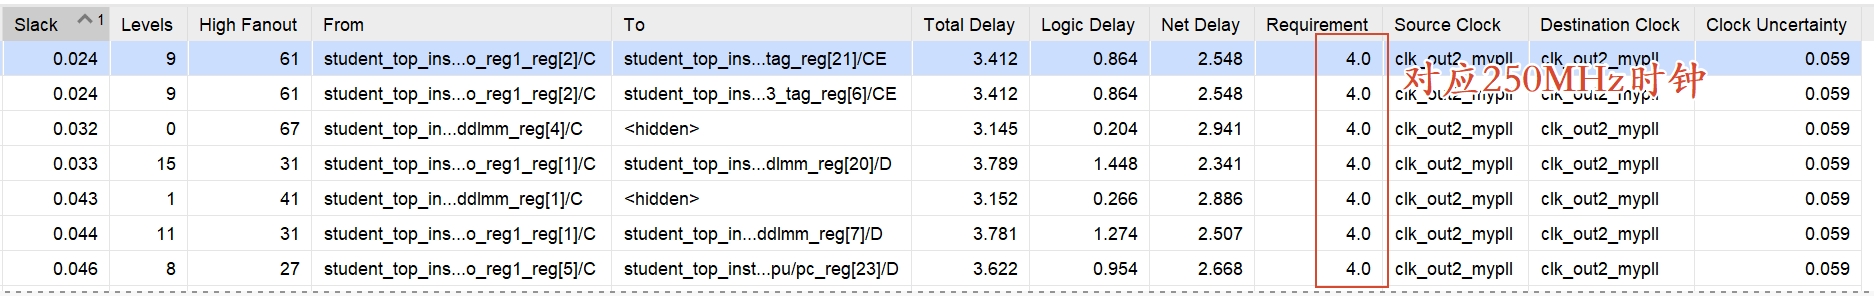
\includegraphics[width=1\linewidth]{imagea.png}
\end{figure}

   CPU 内核采用 IFU--IDU--EXU--LSU--WBU 五级流水顺序单发射架构，配合寄存器旁路、停顿控制、BTB 与 BTFN 静态分支预测，实现了 RV32I 指令与部分 CSR 扩展。

   FPGA 侧使用 Block RAM IP 替代模板提供的 Distributed RAM 作为 IROM、DRAM 的例化，并为此重写了外设桥以适配时序。

\newpage
\endgroup

\section{项目概述}

\subsection{项目背景}

``竞业达''企业命题要求参赛队伍完成一款能够在指定 FPGA 平台上运行的
RISC-V CPU，并最终在``竞业达''官方定制 FPGA
平台上板验证。围绕这一目标，本项目完成了
CPU 内核与简易 SoC 设计，将赛方测试程序配置到板端 IROM/DRAM
并成功完成最终运行。

\subsection{设计目标}

本项目的设计目标包括：实现支持 RV32I 指令集的 RISC-V 处理器；完成
IROM、DRAM 和 MMIO 的统一地址映射；在 FPGA 顶层接入
LED、数码管和计数器等板级资源；保证最终版工程能够在 Vivado 2024
下完成实现，并通过数字孪生平台完成 src0、src1、src2 与 test\_src
四组程序的上板验证。

\subsection{设计平台说明}

本设计使用 Vivado 2024.2 版本进行综合、实现。

硬件平台为``竞业达''官方基于 Kintex-7 定制的 FPGA 开发板，CPU
核心工作频率为 250 MHz。

采用 SystemVerilog 语言进行设计，并使用了 Chisel
完成部分模块的辅助生成，以提高设计抽象层次与开发效率。

\section{RISC-V CPU架构设计}

\subsection{RV32I指令集的支持情况}

项目已支持 RV32I
所有37条整数指令，已经实现整数运算、立即数运算、访存、分支跳转、高位立即数以及部分
CSR/异常返回路径。

\begin{threelongtable}{@{}
  >{\raggedright\arraybackslash}p{(\linewidth - 4\tabcolsep) * \real{0.2}}
  >{\raggedright\arraybackslash}p{(\linewidth - 4\tabcolsep) * \real{0.4}}
  >{\raggedright\arraybackslash}p{(\linewidth - 4\tabcolsep) * \real{0.4}}@{}}
\caption{RV32I 指令支持情况}\\
\toprule\noalign{}
\begin{minipage}[b]{\linewidth}\centering
\textbf{类别}
\end{minipage} & \begin{minipage}[b]{\linewidth}\centering
\textbf{典型指令/功能}
\end{minipage} & \begin{minipage}[b]{\linewidth}\centering
\textbf{说明}
\end{minipage} \\
\midrule\noalign{}
\endhead
\bottomrule\noalign{}
\endlastfoot
寄存器运算 & ADD, SUB, SLL, SLT, SLTU, XOR, SRL, SRA, OR, AND &
由 EXU 中 ALU 完成 \\
立即数运算 & ADDI, SLTI, SLTIU, XORI, ORI, ANDI, SLLI, SRLI/SRAI & 由
IDU 生成立即数，EXU 送入 ALU 完成 \\
访存指令 & LB, LH, LW, LBU, LHU, SB, SH, SW & EXU 生成读写请求，LSU/WBU
完成读结果处理 \\
控制流 & BEQ, BNE, BLT, BGE, BLTU, BGEU, JAL, JALR & EXU
中判定分支预测正误并拉起重定向PC信号 \\
高位立即数 & LUI, AUIPC & 直接形成写回数据 \\
系统相关 & CSRRW, CSRRS, ECALL, MRET & CSR 堆与异常返回已实现 \\
\end{threelongtable}

\subsection{RV32I CPU的整体架构图}

CPU
内核由取指（IFU）、译码（IDU）、执行与访存发起（EXU）、访存响应（LSU）和
写回（WBU）五个主要阶段组成；同时设置独立的寄存器堆、CSR
堆、分支目标缓存和外设桥。对竞业达平台的适配主要体现在 FPGA
顶层的存储器封装和外设桥 MMIO 地址映射。

% \begin{figure}[htbp]
% \centering
% 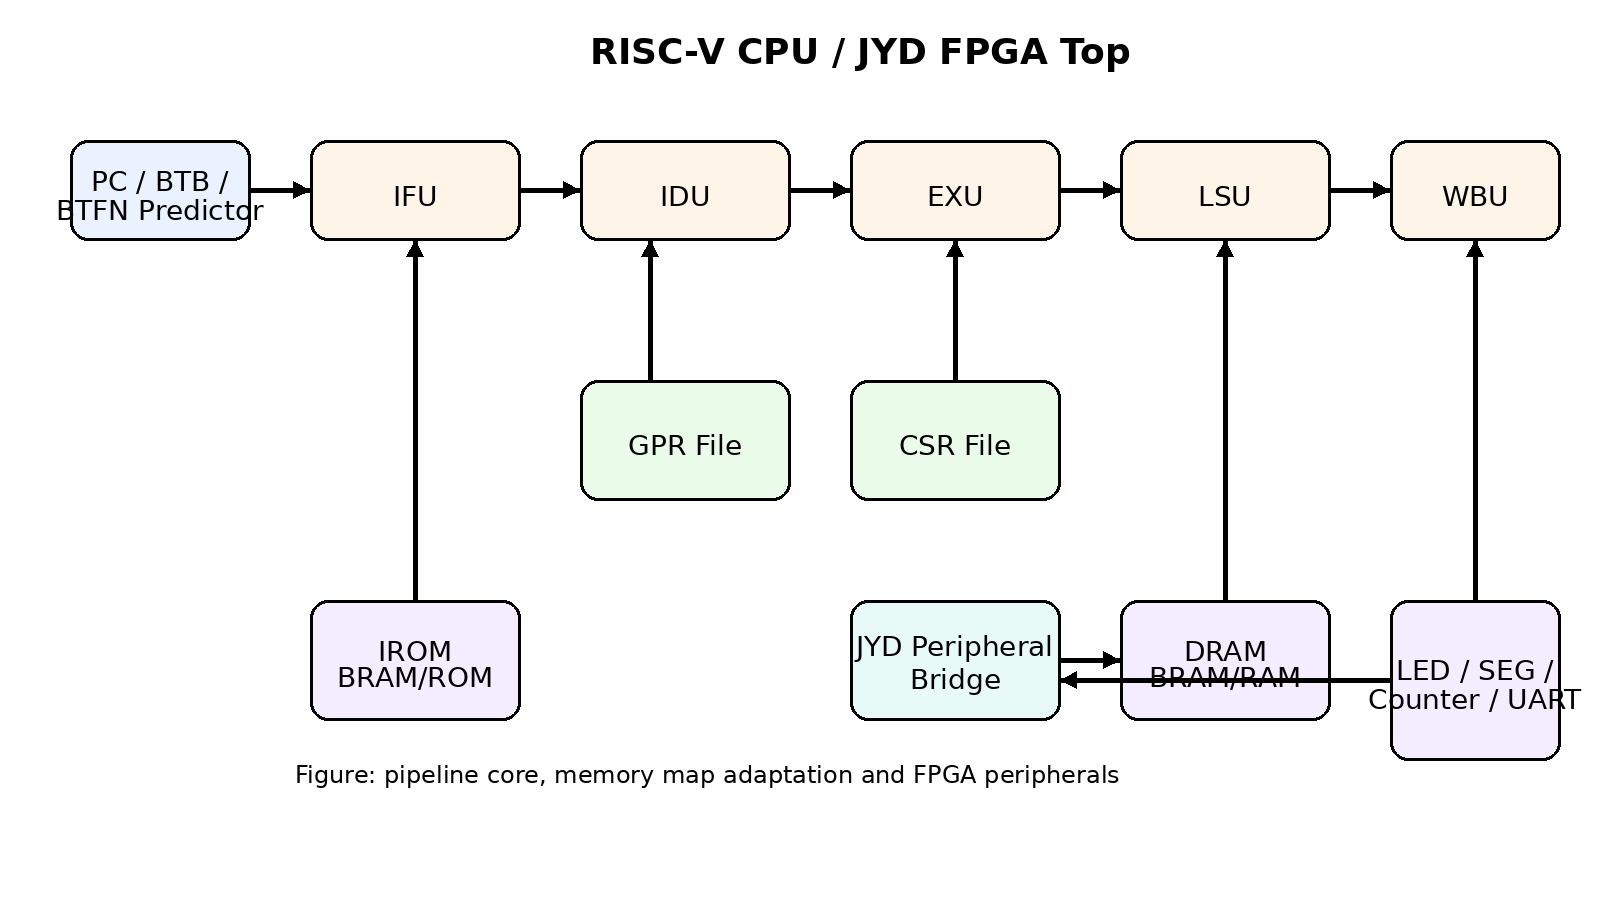
\includegraphics[width=0.96\linewidth]{image4.png}
% \caption{CPU核心与竞业达 FPGA 顶层适配关系示意图}
% \end{figure}

\begin{figure}[htbp]
  \centering
	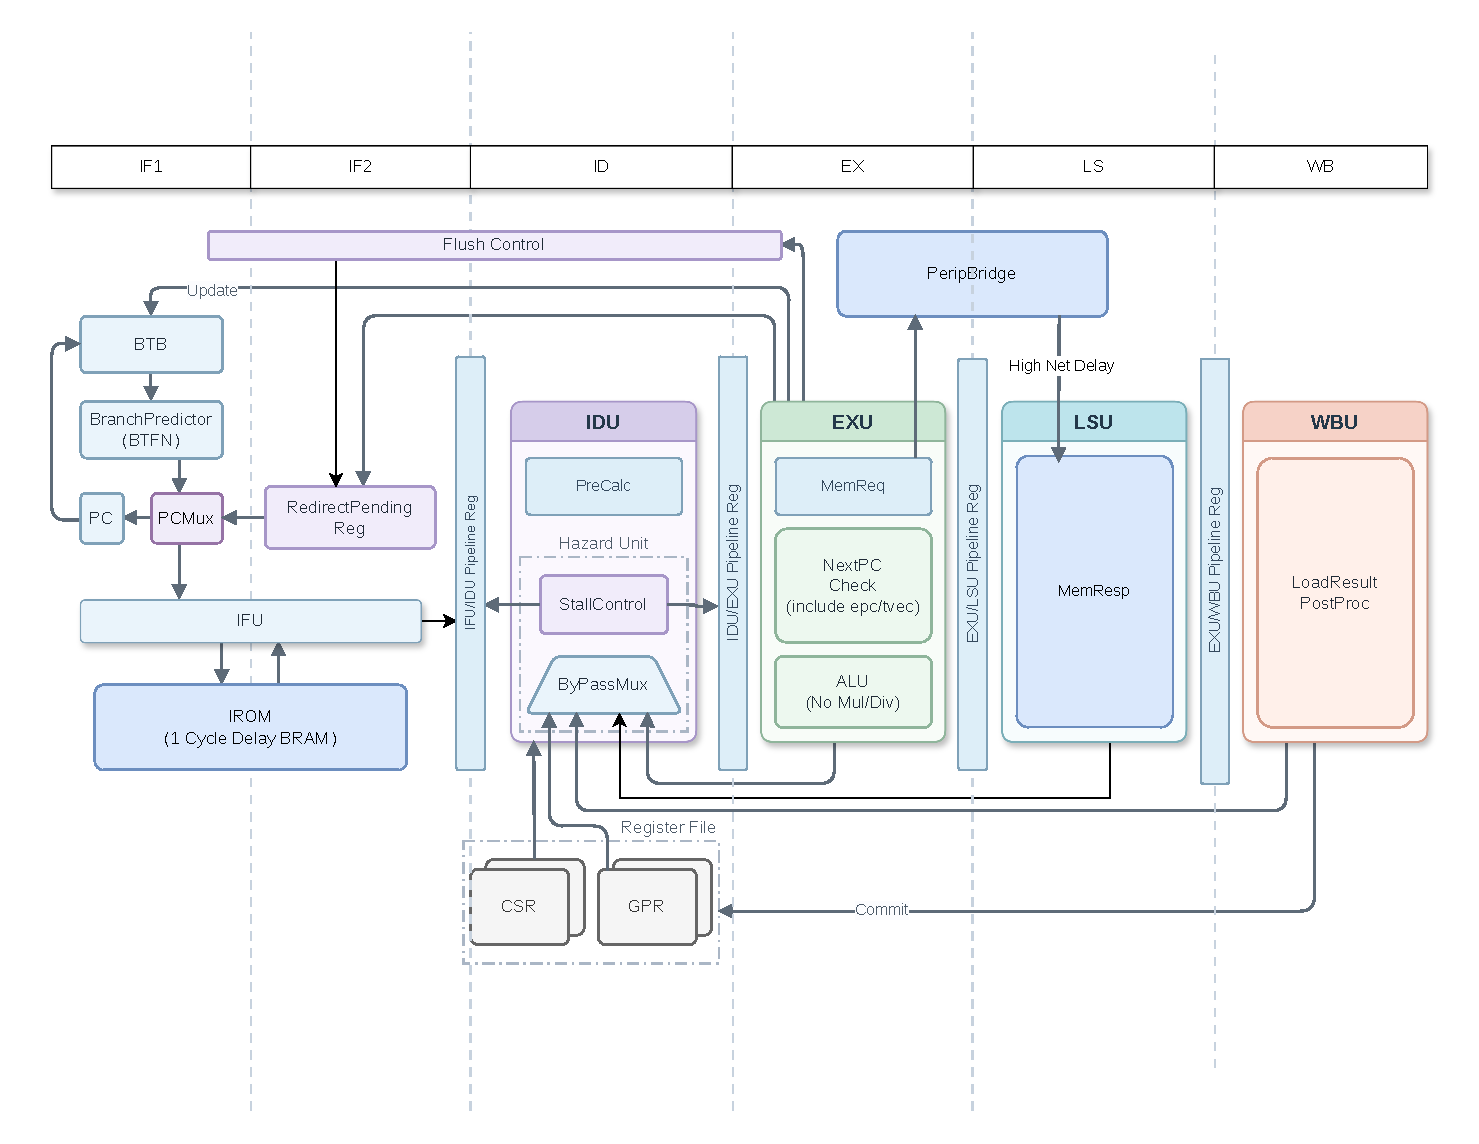
\includegraphics[width=\textwidth]{cpu-arch.pdf}
	\caption{CPU核心与竞业达 FPGA 顶层适配关系示意图}
\end{figure}

\subsection{数据通路各模块的设计}

CPU
数据通路遵循``指令在流水线中逐级传递、控制信息与数据信息同时随指令流动''的设计思路。各模块的职责如下。

\subsubsection{IFU 取指模块}

IFU 作为前端取指单元，负责将 PC 转化为实际取指请求并输出带有
PC、预测信息和指令编号的 FetchedInst，并尽可能保持每周期连续取指。

\begingroup
\setlength\LTleft{\fill}
\setlength\LTright{\fill}
\small
\renewcommand{\arraystretch}{1.2}
\begin{longtable}{@{}
  >{\raggedright\arraybackslash}p{(\linewidth - 4\tabcolsep) * \real{0.2}}
  >{\raggedright\arraybackslash}p{(\linewidth - 4\tabcolsep) * \real{0.1}}
  >{\raggedright\arraybackslash}p{(\linewidth - 4\tabcolsep) * \real{0.7}}@{}}
\caption{IFU 接口信号说明}\\
\toprule\noalign{}
\begin{minipage}[b]{\linewidth}\raggedright
接口
\end{minipage} & \begin{minipage}[b]{\linewidth}\raggedright
方向
\end{minipage} & \begin{minipage}[b]{\linewidth}\raggedright
作用
\end{minipage} \\
\midrule\noalign{}
\endhead
\bottomrule\noalign{}
\endlastfoot
pc & 输入 & 上游给出的待取指地址 \\
predNext & 输入 & 该条指令对应的预测元信息 \\
mem & 输出 & 对取指存储端口发起 SimpleBus 读请求 \\
out & 输出 & 向 IDU 输出 FetchedInst \\
\end{longtable}
\endgroup

其中 FetchedInst 除指令本身外，还携带：当前 pc、预测信息
pred、单调递增的 指令编号 iid。

当前实现使用 4
个状态的状态机处理请求、等待和反压节拍。状态分别为空闲（Idle）、等待访存接受请求（WaitReq）、等待访存返回数据（WaitResp）、等待后级反压结束可以接受新指令数据（WaitOut）。

% https://q.uiver.app/#q=WzAsNyxbMCwwLCJcXHRleHR7SWRsZX0iXSxbMCwyLCJcXHRleHR7V2FpdFJlcX0iXSxbNiwyLCJcXHRleHR7V2FpdFJlc3B9Il0sWzYsMCwiXFx0ZXh0e1dhaXRPdXR9Il0sWzAsMSwiXFxidWxsZXQiXSxbMywwLCJcXGNpcmMiXSxbMywyLCJcXGNpcmMiXSxbNCwwLCJcXHRleHRybXtSZXNldH0iXSxbMiw1LCJcXHRleHRybXtNRU0gYWNjZXB0ZWR9IiwxLHsic3R5bGUiOnsiaGVhZCI6eyJuYW1lIjoiZXBpIn19fV0sWzUsMCwiXFx0ZXh0cm17Tm8gbmV3IHZhbGlkIFBDfSJdLFs1LDYsIlxcdGV4dHJte0hhcyBuZXcgUEN9IiwxLHsic3R5bGUiOnsiaGVhZCI6eyJuYW1lIjoiZXBpIn19fV0sWzYsMiwiXFx0ZXh0cm17TUVNIGFjY2VwdGVkfSIsMV0sWzYsMSwiXFx0ZXh0cm17TUVNIG5vdCByZWFkeX0iLDIseyJvZmZzZXQiOjF9XSxbMSw2LCJcXHRleHRybXtNRU0gYWNjZXB0ZWR9IiwyLHsib2Zmc2V0IjoxLCJzdHlsZSI6eyJoZWFkIjp7Im5hbWUiOiJlcGkifX19XSxbMyw1LCJcXHRleHRybXtPdXQgcmVhZHl9IiwwLHsic3R5bGUiOnsiaGVhZCI6eyJuYW1lIjoiZXBpIn19fV0sWzAsNSwiXFx0ZXh0cm17SGFzIG5ldyBQQ30iLDAseyJvZmZzZXQiOi0yLCJzdHlsZSI6eyJoZWFkIjp7Im5hbWUiOiJlcGkifX19XSxbNSwzLCJcXHRleHRybXtPdXQgbm90IHJlYWR5fSIsMCx7Im9mZnNldCI6LTJ9XV0=
\begin{figure}[htbp]
\centering
\begin{tikzcd}
	{\text{Idle}} &&& \circ &&& {\text{WaitOut}} \\
	\bullet \\
	{\text{WaitReq}} &&& \circ &&& {\text{WaitResp}}
	\arrow["{\textrm{Has new PC}}", shift left=2, two heads, from=1-1, to=1-4]
	\arrow["{\textrm{No new valid PC}}", from=1-4, to=1-1]
	\arrow["{\textrm{Out not ready}}", shift left=2, from=1-4, to=1-7]
	\arrow["{\textrm{Has new PC}}"{description}, two heads, from=1-4, to=3-4]
	\arrow["{\textrm{Out ready}}", two heads, from=1-7, to=1-4]
	\arrow["{\textrm{Reset}}", from=2-1, to=1-1]
	\arrow["{\textrm{MEM accepted}}"', shift right, two heads, from=3-1, to=3-4]
	\arrow["{\textrm{MEM not ready}}"', shift right, from=3-4, to=3-1]
	\arrow["{\textrm{MEM accepted}}"{description}, from=3-4, to=3-7]
	\arrow["{\textrm{MEM accepted}}"{description}, two heads, from=3-7, to=1-4]
\end{tikzcd}
\caption{IFU 状态机的简化状态转移图}
\end{figure}

其中 $\circ$ 表示MUX选择而非状态，具体的状态转移布尔表达式见下图

% https://q.uiver.app/#q=WzAsNSxbMSwwLCJcXHRleHR7SWRsZX0iXSxbMCw0LCJcXHRleHR7V2FpdFJlcX0iXSxbMCwwLCJcXGJ1bGxldCJdLFs3LDAsIlxcdGV4dHtXYWl0UmVzcH0iXSxbOCw0LCJcXHRleHR7V2FpdE91dH0iXSxbMCwxLCJcXHJtIFZhbGlkX3tQQ30gXFxsYW5kIFxcbG5vdCBSZWFkeV97bWVtLnJlcX0iLDJdLFswLDAsIlxcbG5vdCBcXHJtIFZhbGlkX3tQQ30iXSxbMiwwXSxbMywwLCJcXHJtIFZhbGlkX3ttZW0ucmVzcH0gXFxsYW5kIFJlYWR5X3tvdXR9XFxsYW5kXFxsbm90IFZhbGlkX3tQQ30iLDAseyJvZmZzZXQiOi0xfV0sWzAsMywiXFxybSBWYWxpZF97UEN9IFxcbGFuZCBSZWFkeV97bWVtLnJlcX0iLDAseyJvZmZzZXQiOi0xfV0sWzQsMCwiXFxybSBSZWFkeV97b3V0fSBcXGxhbmQgXFxsbm90IFZhbGlkX3tQQ30iLDEseyJsYWJlbF9wb3NpdGlvbiI6NDB9XSxbMSwzLCJcXHJtIFJlYWR5X3ttZW0ucmVxfSIsMCx7ImxhYmVsX3Bvc2l0aW9uIjo0MCwib2Zmc2V0IjoxfV0sWzEsMSwiXFxybSBcXGxub3QgUmVhZHlfe21lbS5yZXF9IiwwLHsiYW5nbGUiOi0xODB9XSxbMywxLCJcXHJte1ZhbGlkX3ttZW0ucmVzcH0gXFxsYW5kIFJlYWR5X3tvdXR9fVxcbGFuZCBWYWxpZF97UEN9IFxcbGFuZCBcXGxub3QgUmVhZHlfe21lbS5yZXF9IiwwLHsib2Zmc2V0IjotM31dLFs0LDEsIlxccm0gUmVhZHlfe291dH1cXGxhbmQgVmFsaWRfe1BDfVxcbGFuZCBcXGxub3QgUmVhZHlfe21lbS5yZXF9IiwwLHsib2Zmc2V0IjotMX1dLFszLDQsIlxccm0gVmFsaWRfe21lbS5yZXNwfSBcXGxhbmQgXFxsbm90IFJlYWR5X3tvdXR9Il0sWzMsMywiXFxybVxcbG5vdCBWYWxpZF97bWVtLnJlc3B9IFxcbG9yICggUmVhZHlfe291dH1cXGxhbmQgVmFsaWRfe1BDfSBcXGxhbmQgUmVhZHlfe21lbS5yZXF9KSJdLFs0LDMsIlxccm0gUmVhZHlfe291dH1cXGxhbmQgVmFsaWRfe1BDfVxcbGFuZCBSZWFkeV97bWVtLnJlcX0iLDEseyJsYWJlbF9wb3NpdGlvbiI6ODAsIm9mZnNldCI6LTJ9XSxbNCw0LCJcXHJtIFxcbG5vdCBSZWFkeV97b3V0fSIsMCx7ImFuZ2xlIjoxODB9XV0=
\begin{figure}[htbp]
\centering
\begin{tikzcd}
	\bullet & {\text{Idle}} &&&&&& {\text{WaitResp}} \\
	\\
	\\
	\\
	{\text{WaitReq}} &&&&&&&& {\text{WaitOut}}
	\arrow[from=1-1, to=1-2]
	\arrow["{\lnot \rm Valid_{PC}}", from=1-2, to=1-2, loop, in=55, out=125, distance=10mm]
	\arrow["{\rm Valid_{PC} \land Ready_{mem.req}}", shift left, from=1-2, to=1-8]
	\arrow["{\rm Valid_{PC} \land \lnot Ready_{mem.req}}"', from=1-2, to=5-1]
	\arrow["{\rm Valid_{mem.resp} \land Ready_{out}\land\lnot Valid_{PC}}", shift left, from=1-8, to=1-2]
	\arrow["{\rm\lnot Valid_{mem.resp} \lor ( Ready_{out}\land Valid_{PC} \land Ready_{mem.req})}", from=1-8, to=1-8, loop, in=55, out=125, distance=10mm]
	\arrow["{\rm{Valid_{mem.resp} \land Ready_{out}}\land Valid_{PC} \land \lnot Ready_{mem.req}}"{pos=0.75}, shift left=3, from=1-8, to=5-1]
	\arrow["{\rm Valid_{mem.resp} \land \lnot Ready_{out}}", from=1-8, to=5-9]
	\arrow["{\rm Ready_{mem.req}}"{pos=0.4}, shift right, from=5-1, to=1-8]
	\arrow["{\rm \lnot Ready_{mem.req}}", from=5-1, to=5-1, loop, in=235, out=305, distance=10mm]
	\arrow["{\rm Ready_{out} \land \lnot Valid_{PC}}"{description, pos=0.4}, from=5-9, to=1-2]
	\arrow["{\rm Ready_{out}\land Valid_{PC}\land Ready_{mem.req}}"{description, pos=0.8}, shift left=2, from=5-9, to=1-8]
	\arrow["{\rm Ready_{out}\land Valid_{PC}\land \lnot Ready_{mem.req}}", shift left, from=5-9, to=5-1]
	\arrow["{\rm \lnot Ready_{out}}", from=5-9, to=5-9, loop, in=235, out=305, distance=10mm]
\end{tikzcd}
\caption{IFU 状态机的完整转移条件}
\end{figure}

若当前周期
IFU 已经准备接受新 PC，但存储端 req\_ready 还未就绪，则
PC 会先进入 pending 路径保存；对应的预测信息和 iid 一并保存；等待后续存储端可接收时再真正发起请求。保证前端不会因为总线短暂背压而丢失刚接到的新负载。

waitResp 状态下若访存响应在当周期返回、且 IDU 也在当周期接收成功，则 IFU
可以立刻接入下一条 PC 并尝试发起下一次请求。
也就是说，下面三件事可以在一个周期中发生： 
消费上一条取指结果；
接收下一条 PC；
发起下一次请求。

从而隐藏了使用BRAM作为 IROM 的一周期延迟，表现出来仍能每周期取指令。

\begin{figure}[htbp]
\centering
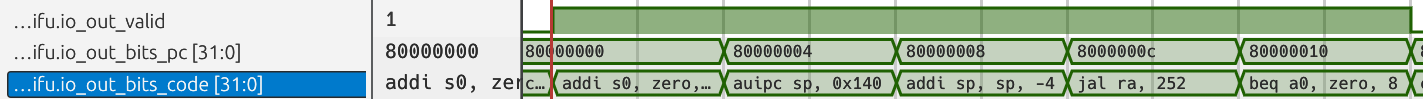
\includegraphics[width=0.96\linewidth]{imaged.png}\\[0.5em]
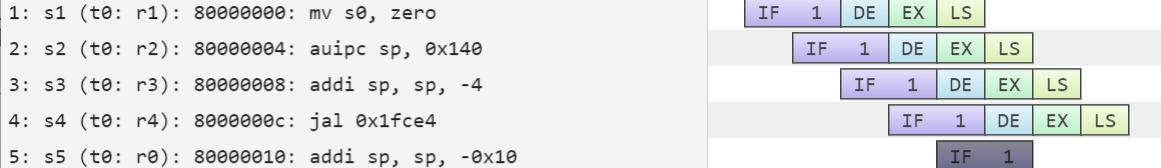
\includegraphics[width=0.88\linewidth]{imagee.png}
\caption{IFU 连续取指与 BRAM 延迟隐藏仿真波形}
\end{figure}

预测结果不在后端重新查询，而是和指令一起进入流水线。这样 EXU
能直接对照该条指令的预测记录做校验，

\subsubsection{IDU 译码与寄存器读取模块}

IDU 包含译码、访问寄存器堆、旁路、预计算功能。

\begin{threelongtable}{@{}
  >{\raggedright\arraybackslash}p{(\linewidth - 4\tabcolsep) * \real{0.2}}
  >{\raggedright\arraybackslash}p{(\linewidth - 4\tabcolsep) * \real{0.1}}
  >{\raggedright\arraybackslash}p{(\linewidth - 4\tabcolsep) * \real{0.7}}@{}}
\caption{IDU 接口信号说明}\\
\toprule\noalign{}
\begin{minipage}[b]{\linewidth}\raggedright
接口
\end{minipage} & \begin{minipage}[b]{\linewidth}\raggedright
方向
\end{minipage} & \begin{minipage}[b]{\linewidth}\raggedright
作用
\end{minipage} \\
\midrule\noalign{}
\endhead
\bottomrule\noalign{}
\endlastfoot
in & 输入 & 来自 IFU 的 FetchedInst \\
rvec & 输出 & 读取两个 GPR 源寄存器 \\
csrRead & 输出 & 读取当前指令需要访问的 CSR \\
csrJmpTarget & 输入 & 提供 mepc/mtvec \\
wrBackInfo & 输入 & 来自 EXU/LSU/WBU 的旁路信息 \\
pipelineFlush & 输入 & 上游通知当前路径是否被清空 \\
out & 输出 & 送往 EXU 的 DecodedInst \\
\end{threelongtable}

译码功能会根据 opcode 将指令粗分为 imm、reg、store、upper、jump、branch
等格式，以及 arithmetic、load、store、jal、jalr、lui、auipc、system
等类型，并生成 I/S/B/U/J 五类立即数，根据指令类型格式选取IMM。

访问寄存器会同时发起双读端口 GPR 访问和单读端口 CSR 访问。

旁路网络通过 \texttt{ByPassMux}
同时观察来自以下三个位置的写回信息：EXU、LSU、WBU

\begin{figure}[htbp]
\centering
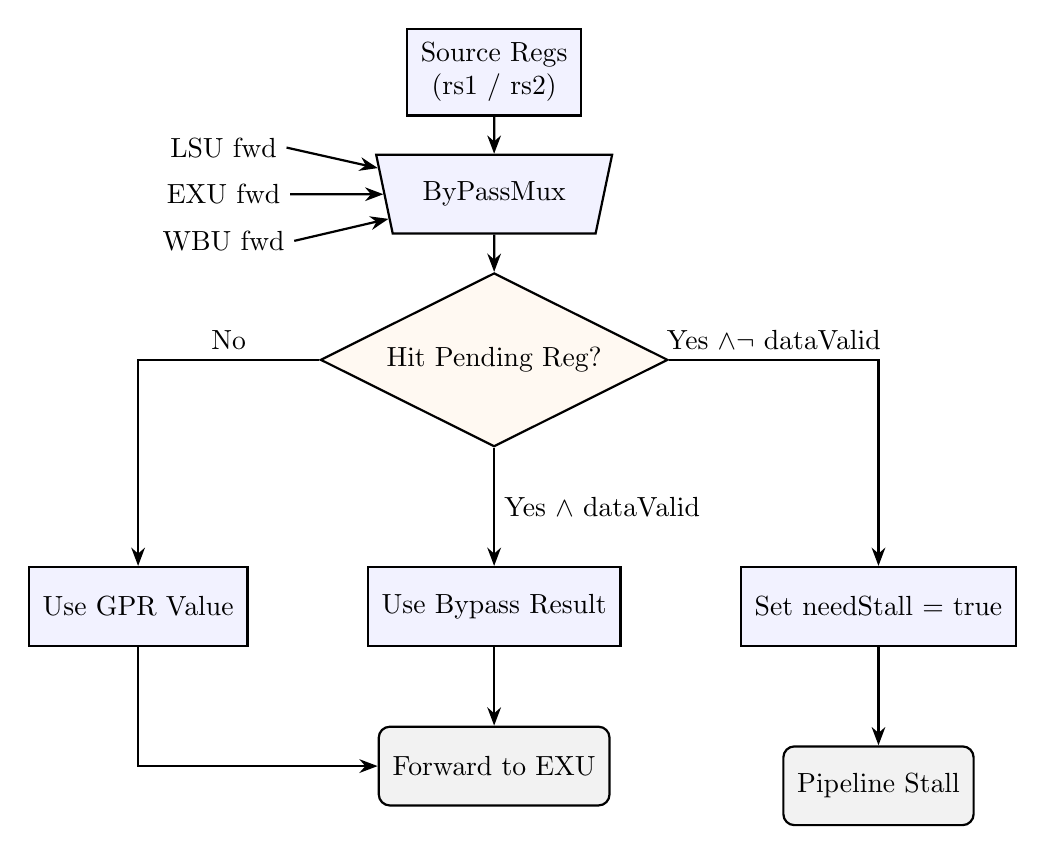
\begin{tikzpicture}[
    node distance=1.5cm and 1cm,
    base/.style={draw,  line width=0.8pt, align=center, minimum height=1cm, inner sep=5pt},
    block/.style={base, rectangle, fill=blue!5},
    decision/.style={base, diamond, aspect=2, fill=orange!5},
    terminal/.style={base, rounded corners, fill=gray!10},
    % 修正梯形定义：
    % 1. trapezium left/right angle 设为相同（如 75 或 80）以保证对称
    % 2. rotate=180 是为了让宽的一边朝上，窄的一边朝下（符合 Mux 逻辑符号习惯）
    mux/.style={base, trapezium, trapezium stretches=true, 
                trapezium left angle=75, trapezium right angle=75, 
                minimum width=3cm, fill=blue!5, rotate=180},
    arrow/.style={-Stealth, thick}
]

    % Nodes
    \node [block] (rs) {Source Regs\\(rs1 / rs2)};
    
    % Mux 节点，内部文字需要配合 rotate 反转回来
    \node [mux] (bpmux) [below=of rs] {\rotatebox{180}{ByPassMux}};
    
    % Forwarding inputs
    \node [left=4cm of bpmux] (exu) {EXU fwd};
    \node [above=0.1cm of exu] (lsu) {LSU fwd};
    \node [below=0.1cm of exu] (wbu) {WBU fwd};

    \node [decision] (conflict) [below=of bpmux] {Hit Pending Reg?};
    
    \node [block] (bypass) [below=of conflict] {Use Bypass Result};
    \node [block] (gpr) [left=1.5cm of bypass] {Use GPR Value};
    \node [block] (stall) [right=1.5cm of bypass] {Set needStall = true};

    \node [terminal] (exu_out) [below=1cm of bypass] {Forward to EXU};
    \node [terminal] (hold) [below=1.25cm of stall] {Pipeline Stall};

    % Path connections
    \draw [arrow] (rs) -- (bpmux);
    
    % 修正箭头重叠：使用具体的 anchor 或偏移量
    % 注意：因为 mux 旋转了180度，原来的 west 变成了现在的 east 视角，
    % 但在 TikZ 坐标中可以直接指定相对于节点的位移
    \draw [arrow] (lsu.east) -- ([yshift=8pt]bpmux);
    \draw [arrow] (exu.east) -- (bpmux);
    \draw [arrow] (wbu.east) -- ([yshift=-8pt]bpmux);
    
    \draw [arrow] (bpmux) -- (conflict);

    % Decision edges
    \draw [arrow] (conflict.west) -| node[above, pos=0.25] {No} (gpr);
    \draw [arrow] (conflict.south) -- node[right] {Yes $\land$ dataValid} (bypass);
    \draw [arrow] (conflict.east) -| node[above, pos=0.25] {Yes $\land\lnot$ dataValid} (stall);

    % Final outputs
    \draw [arrow] (gpr) |- (exu_out);
    \draw [arrow] (bypass) -- (exu_out);
    \draw [arrow] (stall) -- (hold);

\end{tikzpicture}
\caption{IDU 旁路与停顿判定流程}
\end{figure}

旁路的优先级为 EXU > LSU > WBU，当按照优先级顺序检测到源寄存器命中了某个
尚未完成提交的目的寄存器，IDU 会根据该寄存器当前是否持有可用数据（dataValid）做出如下决策：
\begin{itemize}
\item 若该级已经持有可直接转发的数据（dataValid），则直接旁路；
\item 若该级尚无可用数据，则发出停顿。
\end{itemize}

IDU 也会提前计算 PC+4、Reg+IMM、CSRJumpTarget等EXU所需数据减轻EXU时序压力

\subsubsection{EXU 执行模块}

EXU 负责生成当前指令的``真实执行结果''，同时也是控制流分支预测正确性的检测点。
该级从 IDU 接收源操作数、立即数、预测信息以及预先形成的
\texttt{pc+imm}/\texttt{rs1+imm} 等结果，在单拍内完成算术逻辑运算、分支判断、
跳转目标生成、CSR 写控制和访存请求构造，并把后续所需的写回元信息继续传给
LSU/WBU。

\begin{threelongtable}{@{}
  >{\raggedright\arraybackslash}p{(\linewidth - 4\tabcolsep) * \real{0.2}}
  >{\raggedright\arraybackslash}p{(\linewidth - 4\tabcolsep) * \real{0.1}}
  >{\raggedright\arraybackslash}p{(\linewidth - 4\tabcolsep) * \real{0.7}}@{}}
\caption{EXU 接口信号说明}\\
\toprule\noalign{}
\begin{minipage}[b]{\linewidth}\raggedright
接口
\end{minipage} & \begin{minipage}[b]{\linewidth}\raggedright
方向
\end{minipage} & \begin{minipage}[b]{\linewidth}\raggedright
作用
\end{minipage} \\
\midrule\noalign{}
\endhead
\bottomrule\noalign{}
\endlastfoot
in & 输入 & 来自 IDU 的 DecodedInst，包含源操作数、立即数和预测信息 \\
memReq & 输出 & 向数据存储端口发起 load/store 访存请求 \\
out & 输出 & 向 LSU 输出执行结果、访存属性和后续写回元信息 \\
fwd & 输出 & 向 IDU 提供本级可旁路的写回信息 \\
redirectInfo & 输出 & 向顶层提供控制流校验结果与重定向目标 \\
\end{threelongtable}

其核心职责可概括为以下四类：

\begin{itemize}
\item
  \textbf{算术逻辑执行：}对 R-Type、I-Type、LUI、AUIPC 等指令，
  根据译码结果选择 ALU 输入与运算类型，产生寄存器写回值或供后续级继续传递的中间结果。
\item
  \textbf{控制流裁决：}对 BEQ/BNE/BLT/BGE/BLTU/BGEU，
  直接比较当前源操作数并判断分支是否成立；对 JAL/JALR、\texttt{ecall}、
  \texttt{mret}，选择跳转目标，并给出分支 taken 与否。
\item
  \textbf{访存请求前推：}对 load/store 指令，使用 IDU 预先计算好的
  \texttt{rs1+imm} 形成目标地址，并在本级构造访存请求。对 store，写掩码和按地址偏移移位后的写数据也在本级形成；
	对 load，本级只发起读请求。对于 BRAM 等单周期响应的存储器，可以使得下周期 LSU 能够直接拿到数据
	隐藏一周期访存延迟。
\item
  \textbf{写回与前递信息封装：}
  会把目的寄存器号、是否写回、CSR 写控制等信息与执行结果一起向后传递。对非访存类指令，结果通常已在本级可用，可直接参与旁路；对 load
  指令，由于最终返回值要等 LSU/WBU 处理完成，因此不能在本级宣布数据就绪（dataValid）。
\end{itemize}

当 EXU 发现条件分支方向与预测不一致，或者执行到 JALR、\texttt{ecall}、
\texttt{mret} 等预测未支持，需要以后端结果为准的控制转移指令时，
会输出重定向请求和正确目标地址，由顶层统一完成流水线冲刷与 PC 纠正。

\subsubsection{LSU 访存结果整理模块}

LSU 在当前设计中不是重新发起请求的复杂访存控制器，而是承接 EXU
已发起的访存语义，把返回数据与执行级传下来的写回元信息重新组织，再统一送往
WBU。

\begin{threelongtable}{@{}
  >{\raggedright\arraybackslash}p{(\linewidth - 4\tabcolsep) * \real{0.2}}
  >{\raggedright\arraybackslash}p{(\linewidth - 4\tabcolsep) * \real{0.1}}
  >{\raggedright\arraybackslash}p{(\linewidth - 4\tabcolsep) * \real{0.7}}@{}}
\caption{LSU 接口信号说明}\\
\toprule\noalign{}
\begin{minipage}[b]{\linewidth}\raggedright
接口
\end{minipage} & \begin{minipage}[b]{\linewidth}\raggedright
方向
\end{minipage} & \begin{minipage}[b]{\linewidth}\raggedright
作用
\end{minipage} \\
\midrule\noalign{}
\endhead
\bottomrule\noalign{}
\endlastfoot
in & 输入 & 来自 EXU 的访存元信息与预构造写回信息 \\
memResp & 输入 & 来自数据存储端口的读响应数据 \\
out & 输出 & 向 WBU 输出统一格式的写回信息 \\
fwd & 输出 & 向 IDU 提供 LSU 阶段的旁路可用性信息 \\
\end{threelongtable}

LSU 的主要工作包括：

\begin{itemize}
\item
  \textbf{非访存指令透传：}若当前指令不是 load/store，LSU
  基本只对 EXU 传下来的写回信息做流水寄存和继续传递，不重新解释执行语义。
\item
  \textbf{访存结果整理：}对 load/store 指令，LSU 结合 EXU
  已经准备好的地址低位、\texttt{func3} 和写回控制，与存储端口返回的原始 32
  位读数据进行封装，形成统一的写回数据。
\item
  \textbf{旁路有效性区分：}对普通算术结果，前级通常已能给出可直接旁路的数据，LSU 会
	使 dataValid 旁路上级数据；但对
  load 指令，LSU 只拿到了尚未完成字节/半字抽取和符号扩展的原始读数据，
	会置 dataValid 为假，使 IDU 的 load-use 旁路能够判定停顿。
\end{itemize}

\subsubsection{WBU 写回模块}

WBU 是当前五级流水中的最终写回级，负责把前级传来的结果进行最终处理并进行寄存器堆的状态更新。对普通算术、跳转和 CSR 指令，WBU
直接完成最终寄存器/CSR 提交；对 load 指令，WBU
在真正写回前完成最后一步数据位扩展。

\begin{threelongtable}{@{}
  >{\raggedright\arraybackslash}p{(\linewidth - 4\tabcolsep) * \real{0.2}}
  >{\raggedright\arraybackslash}p{(\linewidth - 4\tabcolsep) * \real{0.1}}
  >{\raggedright\arraybackslash}p{(\linewidth - 4\tabcolsep) * \real{0.7}}@{}}
\caption{WBU 接口信号说明}\\
\toprule\noalign{}
\begin{minipage}[b]{\linewidth}\raggedright
接口
\end{minipage} & \begin{minipage}[b]{\linewidth}\raggedright
方向
\end{minipage} & \begin{minipage}[b]{\linewidth}\raggedright
作用
\end{minipage} \\
\midrule\noalign{}
\endhead
\bottomrule\noalign{}
\endlastfoot
in & 输入 & 来自 LSU 的统一写回信息 \\
gpr & 输出 & 对 GPR 文件发起最终写回 \\
csr & 输出 & 对 CSR 文件发起最终写回 \\
fwd & 输出 & 向 IDU 提供最可靠的最终旁路结果 \\
\end{threelongtable}

WBU 的关键职责如下：

\begin{itemize}
\item
  \textbf{普通写回提交：}对非 load 指令，WBU
  直接根据前级给出的寄存器写回控制和 CSR 写控制，更新 GPR/CSR 状态。
\item
  \textbf{load 数据重组：}对 LB/LH/LW/LBU/LHU，WBU
  根据地址低位偏移从 \texttt{lsuResult} 中取出目标字节、半字或整字，再依据
  \texttt{func3} 决定是否做符号扩展。把这一步放在最后一级以减轻 LSU
  的时序压力。
\item
  \textbf{最终旁路输出：}WBU
  给出的结果已经是最终写回值,可始终作为旁路网络中最可靠的数据来源（dataValid 始终为 1)。
\end{itemize}

\subsubsection{GPR 与 CSR 模块}

寄存器文件部分由通用寄存器堆 GPR 与控制状态寄存器堆 CSR
共同组成，负责维护当前处理器最核心的体系结构状态。前者服务于 RV32I
数据通路中的通用寄存器读写，后者承担最小机器态控制、陷入返回和计数功能。

\begin{threelongtable}{@{}
  >{\raggedright\arraybackslash}p{(\linewidth - 4\tabcolsep) * \real{0.15}}
  >{\raggedright\arraybackslash}p{(\linewidth - 4\tabcolsep) * \real{0.25}}
  >{\raggedright\arraybackslash}p{(\linewidth - 4\tabcolsep) * \real{0.6}}@{}}
\caption{GPR 接口信号说明}\\
\toprule\noalign{}
\begin{minipage}[b]{\linewidth}\raggedright
GPR 接口
\end{minipage} & \begin{minipage}[b]{\linewidth}\raggedright
方向
\end{minipage} & \begin{minipage}[b]{\linewidth}\raggedright
作用
\end{minipage} \\
\midrule\noalign{}
\endhead
\bottomrule\noalign{}
\endlastfoot
read & 输入地址/输出数据 & 提供两个读端口，供 IDU 读取 rs1/rs2 \\
write & 输入 & 提供一个写端口，供 WBU 提交 rd 写回结果 \\
\end{threelongtable}

\begin{threelongtable}{@{}
  >{\raggedright\arraybackslash}p{(\linewidth - 4\tabcolsep) * \real{0.15}}
  >{\raggedright\arraybackslash}p{(\linewidth - 4\tabcolsep) * \real{0.25}}
  >{\raggedright\arraybackslash}p{(\linewidth - 4\tabcolsep) * \real{0.6}}@{}}
\caption{CSR 接口信号说明}\\
\toprule\noalign{}
\begin{minipage}[b]{\linewidth}\raggedright
CSR 接口
\end{minipage} & \begin{minipage}[b]{\linewidth}\raggedright
方向
\end{minipage} & \begin{minipage}[b]{\linewidth}\raggedright
作用
\end{minipage} \\
\midrule\noalign{}
\endhead
\bottomrule\noalign{}
\endlastfoot
read & 输入地址/输出数据 & 供 IDU 读取当前指令需要访问的 CSR \\
write & 输入 & 供 WBU 提交 CSR 写回地址与数据 \\
is\_ecall & 输入 & 标识当前写回项是否需要触发 \texttt{ecall} 相关语义 \\
mepc/mtvec & 输出 & 为 \texttt{mret}/\texttt{ecall} 提供控制流目标 \\
mcycle64 & 输出 & 提供周期计数信息 \\
\end{threelongtable}

GPR 文件采用双读单写结构，满足大多数 RV32I
指令``双源一目的''的操作数需求。其实现中始终保证 \texttt{x0}
硬连线为零：读 \texttt{x0} 必定得到 0，对 \texttt{x0}
的写请求会被忽略，不会改变寄存器堆内容。

当前 CSR 的支持是满足使 RT-Thread 运行的子集，非完整的异常/中断体系。
提供了下述寄存器的支持：
\texttt{mstatus}、\texttt{mtvec}、\texttt{mepc}、\texttt{mcause}、
\texttt{mcycle}、\texttt{mcycleh}、\texttt{mvendorid} 和
\texttt{marchid}。其中与控制流最直接相关的行为为：

\begin{itemize}
\item
  \texttt{mcycle}\texttt{/}\texttt{mcycleh} 随时钟递增，用于提供最基本的周期计数。
\item
  \texttt{ecall} 提交时把当前 \texttt{pc} 写入 \texttt{mepc}，并把
  \texttt{mcause} 置为 11。
\item
  \texttt{mret} 执行时根据 \texttt{mepc} 恢复控制流。
\end{itemize}

CPU 已经具备最基本的自陷与返回能力，但尚未扩展到完整的机器态控制语义。

\subsubsection{分支预测与控制流修正}

当前 CPU 的分支预测子系统由跳转目标表（BranchTargetBuffer, BTB） 和
分支预测器（BranchPredictor, BP） 组成， BTB
负责记录历史目标地址及其关键属性，预测器则基于这些记录决定下一拍是否沿预测目标继续取指。

\begin{threelongtable}{@{}
  >{\raggedright\arraybackslash}p{(\linewidth - 4\tabcolsep) * \real{0.1}}
  >{\raggedright\arraybackslash}p{(\linewidth - 4\tabcolsep) * \real{0.2}}
  >{\raggedright\arraybackslash}p{(\linewidth - 4\tabcolsep) * \real{0.7}}@{}}
\caption{分支预测与重定向接口说明}\\
\toprule\noalign{}
\begin{minipage}[b]{\linewidth}\raggedright
信号
\end{minipage} & \begin{minipage}[b]{\linewidth}\raggedright
方向
\end{minipage} & \begin{minipage}[b]{\linewidth}\raggedright
作用
\end{minipage} \\
\midrule\noalign{}
\endhead
\bottomrule\noalign{}
\endlastfoot
pc & 输入 & 输入当前待预测的取指地址，用于 BTB 查询 \\
pred & 输出 & 输出预测结果，包含是否命中、是否预测跳转和预测目标 \\
update & 输入 & 接收 EXU 给出的真实控制流结果，用于更新 BTB 表项 \\
redirect & 输入/输出 & 表示当前是否需要修正前端 PC，并携带修正目标 \\
\end{threelongtable}

BTB 采用了参数化的直接映射结构，索引和标记字段的划分基于表项数 \(N\) 和指令地址的位宽。
采用直接映射组织。若记表项数为 \(N\)，则索引和标记字段为：
\[\text{index} = \mathtt{pc}\lbrack\log_{2}N + 1:2\rbrack\]
\[\text{tag} = \mathtt{pc}\lbrack 31:\log_{2}N + 2\rbrack\]

每个表项记录 \texttt{valid}、\texttt{tag}、\texttt{target}、
\texttt{isJAL} 和 \texttt{isBackward} 五类信息。作为当前静态预测需要的最小字段集。

当前 BTB 共有 8 项，即 \(N=8\)，索引字段为 \texttt{pc[4:2]}，标记字段为 \texttt{pc[31:5]}。

BranchPredictor 当前采用静态 BTFN(Backward Taken, Forward Not Taken) 与 JAL 表混合策略：


\begin{itemize}
\item 若 BTB 命中且该项对应 \texttt{JAL}，则直接预测跳转到历史目标。
\item 若 BTB 命中且该项对应后向条件分支，则预测跳转。
\item 其余情况默认预测 \texttt{pc + 4}。
\end{itemize}

\begin{figure}[htbp]
\centering
\resizebox{\linewidth}{!}{%
\begin{tikzpicture}[
    font=\small,
    node distance=1cm and 1.5cm,
    base/.style={draw, line width=0.8pt, align=center, minimum height=0.95cm, inner sep=4pt},
    block/.style={base, rectangle, rounded corners=2pt, fill=blue!5, minimum width=2.5cm},
    decision/.style={base, diamond, aspect=1.8, fill=orange!5, inner sep=0pt, text width=2.1cm},
    arrow/.style={-Stealth, thick, rounded corners=2pt}
]

    % --- 节点定义 ---
    \node [block] (btb) {BTB 查询};
    \node [decision] (hit) [right=of btb] {命中?};
    
    % 上方分支 (命中/预测跳转)
    \node [block] (bp) [above right=0.6cm and 1.5cm of hit] {BranchPredictor};
    \node [decision] (take) [right=of bp] {\texttt{isJAL} 或\\ \texttt{backward}?};
    \node [block] (target) [right=of take] {预测跳转到\\ \texttt{historyTarget}};
    
    % 下方分支 (不命中/顺序执行)
    \node [block] (fall) [below=2cm of target] {预测 \\ \texttt{pc + 4}};
    
    % 汇总部分
    \node [block] (pred) [right=1.5cm of target] {生成 \\ \texttt{PredBundle} \\ 送往 IFU};
    % \node [block] (ifu) [right=of pred] {送往 IFU};

    % --- 连线逻辑 ---
    \draw [arrow] (btb) -- (hit);
    
    % 命中分支 (向上)
    \draw [arrow] (hit) |- node[pos=0.25, left] {是} (bp);
    \draw [arrow] (bp) -- (take);
    \draw [arrow] (take) -- node[above] {是} (target);
    \draw [arrow] (target) -- (pred);
    
    % 不命中分支 (向下)
    \draw [arrow] (hit) |- node[pos=0.25, left] {否} (fall);
    
    % 命中但选择不跳转 (take=否 -> 降至 pc+4)
    % 使用坐标偏移使线条更美观
    \draw [arrow] (take) -- node[pos=0.3, right] {否} (take |- fall.west) -- (fall);
    
    % 汇总连线
    \draw [arrow] (fall) -| (pred);
    % \draw [arrow] (pred) -- (ifu);

\end{tikzpicture}
}
\caption{BTB 与 BTFN 分支预测流程}
\end{figure}

由 BTB 负责在预测跳转时给出目标地址。预测结果会随指令一起进入流水线，
后端 EXU 直接用该条指令携带的预测记录进行校验判定是否预测错误。当前实现中，下列场景会触发重定向：
 \texttt{JALR}；
 \texttt{ecall}\texttt{/}\texttt{mret}；
 条件分支方向与预测不一致；
 \texttt{JAL} 未命中 BTB。

\begin{figure}[htbp]
\centering
\begin{tikzpicture}[
    scale=0.8,
    transform shape,
    node distance=1cm and 1.6cm,
    base/.style={draw, line width=0.8pt, align=center, minimum height=1cm, inner sep=5pt},
    block/.style={base, rectangle, fill=blue!5, minimum width=4.2cm},
    decision/.style={base, diamond, aspect=2, fill=orange!5, inner sep=2pt},
    terminal/.style={base, rounded corners, fill=gray!10, minimum width=4.2cm},
    arrow/.style={-Stealth, thick}
]

    \node [terminal] (exu) {EXU 给出真实控制流结果};
    \node [decision] (jump) [below=of exu] {发生控制转移?};
    \node [block] (update) [below left=of jump] {更新 BTB 表项\\
    \texttt{valid/tag/target}\\
    \texttt{/isJAL/isBackward}};
    \node [terminal] (keep) [below right=of jump] {BTB 保持原状态};

    \node [decision] (wrong) [below=2.8cm of jump] {predWrong?};
    \node [terminal] (ok) [below left=of wrong] {沿当前流水继续执行};
    \node [block] (redirect) [below right=of wrong] {产生 \texttt{redirectNow}\\
    和 \texttt{redirectNowTarget}\\下一周期由顶层重新喂给 IFU};


    \draw [arrow] (exu) -- (jump);
    \draw [arrow] (jump.west) -| node[above, pos=0.25] {是} (update);
    \draw [arrow] (jump.east) -| node[above, pos=0.25] {否} (keep);

    \draw [arrow] (jump) -- (wrong);

    \draw [arrow] (wrong.west) -| node[above, pos=0.25] {否} (ok);
    \draw [arrow] (wrong.east) -| node[above, pos=0.25] {是} (redirect);

\end{tikzpicture}
\caption{后端控制流校验与 BTB 更新流程}
\end{figure}

一旦 EXU 判定需要修正 PC，就产生 \texttt{redirectNow} 和
\texttt{redirectNowTarget}。顶层通过
\texttt{redirectPendingReg} 暂存重定向信息打一拍，下一周期再重新送回 IFU，冲刷惩罚总共 3 个周期。

\begin{figure}[H]
\centering
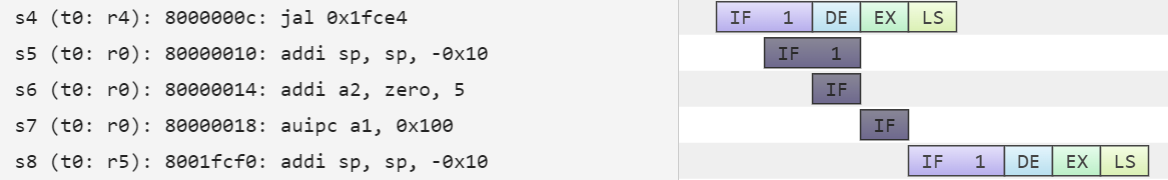
\includegraphics[width=0.96\linewidth]{img_flush.png}
\caption{预测错误后的流水线冲刷}
\end{figure}

\subsubsection{SoC 封装与外设映射模块}

JYDSoC 与 JYDFPGATop 分别是为 CPU 提供用于仿真和上板的运行环境平台封装，使核心 CPU
能够方便的在仿真环境中运行，也能过渡到 FPGA 板级验证。

该平台的主要组成包括 CPUCore、IROM、DRAM、JYDPeripheralBridge，以及
LED、数码管、计数器、UART
等少量 MMIO 外设。两种平台形态的分工如下：

\begin{itemize}
\item
  \textbf{仿真版 JYDSoC：}采用便于初始化和观察的存储器实现，方便快速加载镜像、运行测试并观察外设状态。
\item
  \textbf{FPGA 版 JYDFPGATop：}保持与仿真版一致的地址空间和访问方式，并把 IROM、DRAM 和板级外设替换为实际硬件实现。
\end{itemize}

地址空间采用固定划分：IROM 基址为 \texttt{0x80000000}，DRAM 基址为
\texttt{0x80100000}，MMIO 位于 \texttt{0x80200000}
段。LED、数码管、计数器和 UART
分别占据各自的地址窗口，从而使程序、仿真环境与板级系统在地址视角下保持一致。

其中 JYDPeripheralBridge 是访存的外设桥接模块。它负责根据 CPU
发出的数据访问地址进行译码：默认请求进入 DRAM，命中其他相应窗口时则转发到
LED、SEG、CNT 或 UART（仅仿真使用） 等外设；
同时保留了模板中对计数器跨时钟 CNT 的相关寄存器的相关控制信号。通过把这些平台相关逻辑集中在桥接层，可以在不修改 CPU
核心执行语义的前提下完成仿真版与 FPGA 版平台切换。

在 FPGA 顶层实现中，IROM 和 DRAM 通过 \texttt{blk\_mem\_gen\_xxx}
黑盒接入，计数器通过板级时钟驱动的 counter IP
实现，整体保持与仿真版一致的接口习惯和访问时序。

\begin{figure}[htbp]
\centering
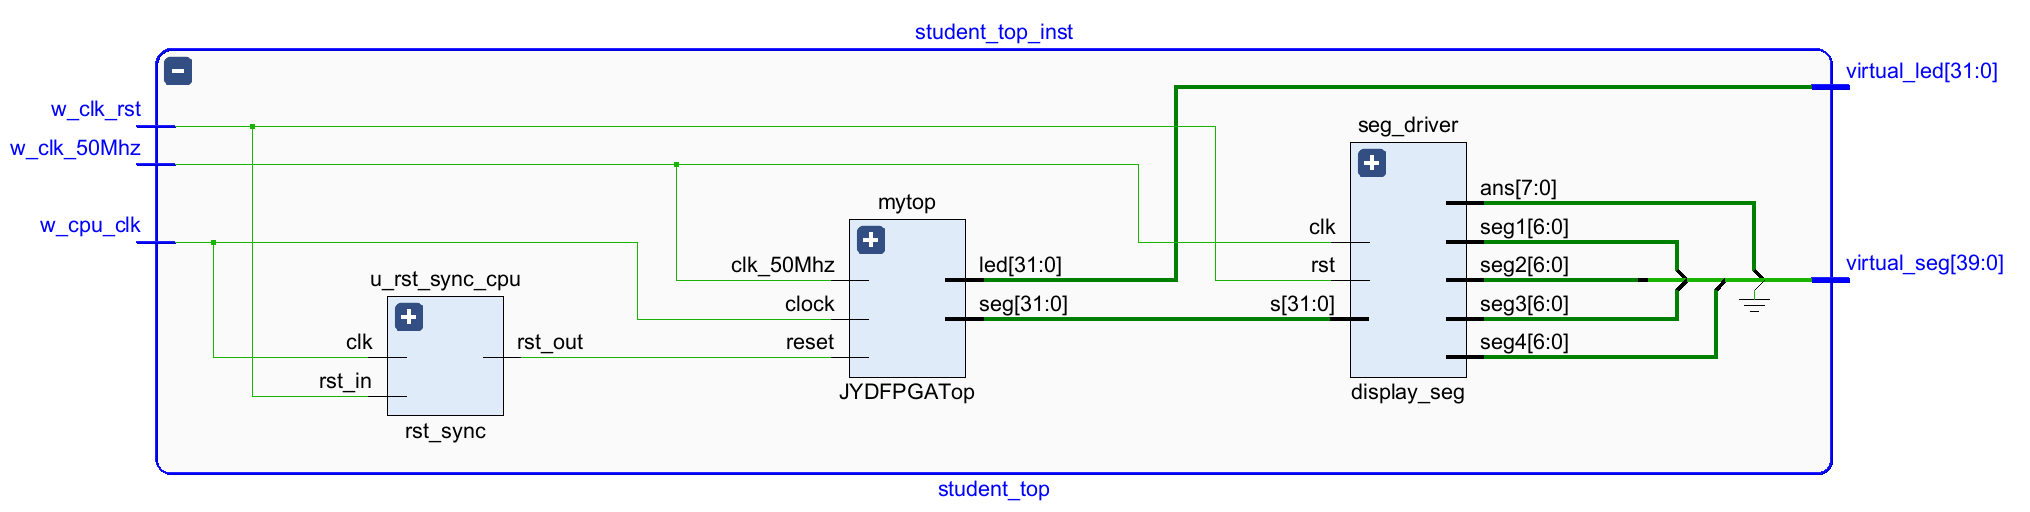
\includegraphics[width=0.96\linewidth]{image7.png}\\[0.6em]

\includegraphics[width=0.96\linewidth]{image8.png}
\caption{JYD SoC 封装与 FPGA 顶层外设映射}
\end{figure}

\subsubsection{内存接口设计}

CPU 核心内部统一采用轻量级的 SimpleBus 风格接口组织取指和数据访存。该接口既能表达只读取指，也能表达 load/store
访问，协议简单，同时又能支持未来可变延迟的外部总线桥接。

\begin{threelongtable}{@{}
  >{\raggedright\arraybackslash}p{(\linewidth - 4\tabcolsep) * \real{0.1}}
  >{\raggedright\arraybackslash}p{(\linewidth - 4\tabcolsep) * \real{0.4}}
  >{\raggedright\arraybackslash}p{(\linewidth - 4\tabcolsep) * \real{0.5}}@{}}
\caption{SimpleBus 字段说明}\\
\toprule\noalign{}
\begin{minipage}[b]{\linewidth}\raggedright
字段类别
\end{minipage} & \begin{minipage}[b]{\linewidth}\raggedright
主要信号
\end{minipage} & \begin{minipage}[b]{\linewidth}\raggedright
作用
\end{minipage} \\
\midrule\noalign{}
\endhead
\bottomrule\noalign{}
\endlastfoot
请求侧 & req\_valid、req\_ready、addr、size、wen、wdata、wmask & 表达一次读/写请求的握手、地址、访存宽度及写数据语义 \\
响应侧 & resp\_valid、rdata & 返回访存完成标志和读数据 \\
\end{threelongtable}

在核心内部，取指路径和数据路径分离：IFU 直接通过一条
SimpleBus 主口访问 IROM；数据访存则由 EXU 产生请求，经
DataMemBusCombiner 统一整理后送往 SoC 的数据口，外部的存储器结构与 CPU 解耦。

DataMemBusCombiner 在这里负载的是数据访存出口整理，将 EXU
发起的 load/store 请求封装到统一的数据总线形式中，并把返回结果再交给流水线后级处理。

\subsection{数据通路信号表}

\begin{threelongtable}{@{}
  >{\raggedright\arraybackslash}p{(\linewidth - 4\tabcolsep) * \real{0.1871}}
  >{\raggedright\arraybackslash}p{(\linewidth - 4\tabcolsep) * \real{0.3441}}
  >{\raggedright\arraybackslash}p{(\linewidth - 4\tabcolsep) * \real{0.4688}}@{}}
\caption{主数据通路总览}\\
\toprule\noalign{}
\begin{minipage}[b]{\linewidth}\raggedright
流向
\end{minipage} & \begin{minipage}[b]{\linewidth}\raggedright
传递内容
\end{minipage} & \begin{minipage}[b]{\linewidth}\raggedright
说明
\end{minipage} \\
\midrule\noalign{}
\endhead
\bottomrule\noalign{}
\endlastfoot
IFU -\textgreater{} IDU & inst、pc、预测信息 & 取指结果进入译码级 \\
IDU -\textgreater{} EXU & imm、src1、src2、地址预计算结果 &
译码级向执行级发送操作数与控制信息 \\
EXU -\textgreater{} LSU & 访存属性、预构造写回信息 & 访存类指令进入 LSU
时将获取读取结果 \\
LSU -\textgreater{} WBU & 原始读数据、写回控制信息 & WBU 完成最终写回 \\
EXU -\textgreater{} 访存接口 &
mem\_addr、mem\_we、mem\_wdata、mem\_wmask & 访存请求从 EXU 发出 \\
WBU -\textgreater{} GPR & rd\_we、rd\_wdata & 最终通用寄存器提交 \\
\end{threelongtable}

U类与J类指令均有写回，写回数据根据指令相关；\texttt{pc\_next} 由 EXU
确定。

\begin{threelongtable}{@{}
  >{\raggedright\arraybackslash}p{(\linewidth - 8\tabcolsep) * \real{0.0583}}
  >{\raggedright\arraybackslash}p{(\linewidth - 8\tabcolsep) * \real{0.3477}}
  >{\raggedright\arraybackslash}p{(\linewidth - 8\tabcolsep) * \real{0.2177}}
  >{\raggedright\arraybackslash}p{(\linewidth - 8\tabcolsep) * \real{0.1210}}
  >{\raggedright\arraybackslash}p{(\linewidth - 8\tabcolsep) * \real{0.2553}}@{}}
\caption{U-Type 与跳转类指令的关键数据通路}\\
\toprule\noalign{}
\begin{minipage}[b]{\linewidth}\raggedright
指令
\end{minipage} & \begin{minipage}[b]{\linewidth}\raggedright
IDU 关键数据通路
\end{minipage} & \begin{minipage}[b]{\linewidth}\raggedright
EXU 关键数据通路
\end{minipage} & \begin{minipage}[b]{\linewidth}\raggedright
写回数据
\end{minipage} & \begin{minipage}[b]{\linewidth}\raggedright
pc\_next / 控制流
\end{minipage} \\
\midrule\noalign{}
\endhead
\bottomrule\noalign{}
\endlastfoot
LUI                                    & {\ttfamily imm = immU}                            & 直接选择立即数通路                                                                               & {\ttfamily imm}        & {\ttfamily pc + 32'd4}                                                     \\
AUIPC                                  & {\ttfamily imm = immU, pc\_plus\_imm = pc + imm}  & 直接选择 \texttt{pc\_plus\_imm}                                                                  &
{\ttfamily pc\_plus\_imm}  & {\ttfamily pc + 32'd4}                \\
JAL                                    & {\ttfamily imm = immJ, pc\_plus\_imm = pc + imm}  & {\ttfamily jump = 1'b1}，跳转目标为 \texttt{pc\_plus\_imm}                                       & {\ttfamily pc + 32'd4} & {\ttfamily pc\_plus\_imm;} 若预测未命中，则 {\ttfamily pred\_wrong = 1'b1} \\
JALR                                   & {\ttfamily imm = immI, addr\_calc = src1 + imm}   & 跳转目标为
{\ttfamily \{addr\_calc[31:1], 1'b0\}} & {\ttfamily pc + 32'd4}                & {\ttfamily \{addr\_calc[31:1], 1'b0\}}；当前实现未对 JALR 做预测，故执行时总会重定向 \\
\end{threelongtable}

分支类指令：IDU 阶段统一完成：\texttt{imm = immB}、\texttt{src1 = rs1}、\texttt{src2 = rs2}、
\texttt{pc\_plus\_imm = pc + immB}；无写回；分支目标统一为
\texttt{branch\_target = pc\_plus\_imm}
（也即 \texttt{pc\_next = branch\_taken ? branch\_target : (pc + 32'd4)}）；预测错误判定方法为预测 Taken 和实际 Taken
不一致（\texttt{pred\_wrong = branch\_taken \^{} pred\_taken}）

比较运算独立于 ALU 单独完成（即未复用 ALU 计算比较）

\begin{threelongtable}{@{}
  >{\centering\arraybackslash}p{(\linewidth - 2\tabcolsep) * \real{0.1004}}
  >{\raggedright\arraybackslash}p{(\linewidth - 2\tabcolsep) * \real{0.7112}}@{}}
\caption{分支类指令的执行条件}\\
\toprule\noalign{}
\begin{minipage}[b]{\linewidth}\centering
指令
\end{minipage} & \begin{minipage}[b]{\linewidth}\raggedright
EXU 分支成立条件 branch\_taken
\end{minipage} \\
\midrule\noalign{}
\endhead
\bottomrule\noalign{}
\endlastfoot
BEQ & {\ttfamily branch\_taken = (src1 == src2)} \\
BNE & {\ttfamily branch\_taken = (src1 != src2)} \\
BLT & {\ttfamily branch\_taken = (\$signed(src1) < \$signed(src2))} \\
BGE & {\ttfamily branch\_taken = !(\$signed(src1) < \$signed(src2))} \\
BLTU & {\ttfamily branch\_taken = (src1 < src2)} \\
BGEU & {\ttfamily branch\_taken = !(src1 < src2)} \\
\end{threelongtable}

Load 类指令：IDU 阶段统一完成：\texttt{imm = immI}、\texttt{addr\_calc = src1 + imm}；EXU 阶段统一发起读请求：\texttt{mem\_addr = addr\_calc}、\texttt{mem\_we = 1'b0}；LSU
阶段统一接收：\texttt{mem\_rdata\_raw}；有写回且写回数据为处理后的访存结果；\texttt{pc\_next = pc + 32'd4}

\begin{threelongtable}{@{}
  >{\raggedright\arraybackslash}p{(\linewidth - 4\tabcolsep) * \real{0.0930}}
  >{\raggedright\arraybackslash}p{(\linewidth - 4\tabcolsep) * \real{0.2110}}
  >{\raggedright\arraybackslash}p{(\linewidth - 4\tabcolsep) * \real{0.6959}}@{}}
\caption{Load 类指令的访存与写回行为}\\
\toprule\noalign{}
\begin{minipage}[b]{\linewidth}\raggedright
指令
\end{minipage} & \begin{minipage}[b]{\linewidth}\raggedright
EXU 访存控制
\end{minipage} & \begin{minipage}[b]{\linewidth}\raggedright
WBU 写回数据
\end{minipage} \\
\midrule\noalign{}
\endhead
\bottomrule\noalign{}
\endlastfoot
LB & {\ttfamily mem\_size = 2'b00} & 从 \texttt{mem\_rdata\_raw} 中按
\texttt{mem\_addr[1:0]} 取 1 字节，并做符号扩展 \\
LH & {\ttfamily mem\_size = 2'b01} & 从 \texttt{mem\_rdata\_raw} 中按
\texttt{mem\_addr[1:0]} 取 2 字节，并做符号扩展 \\
LW & {\ttfamily mem\_size = 2'b10} & {\ttfamily load\_data = mem\_rdata\_raw} \\
LBU & {\ttfamily mem\_size = 2'b00} & 从 \texttt{mem\_rdata\_raw} 中按
\texttt{mem\_addr[1:0]} 取 1 字节，并做零扩展 \\
LHU & {\ttfamily mem\_size = 2'b01} & 从 \texttt{mem\_rdata\_raw} 中按
\texttt{mem\_addr[1:0]} 取 2 字节，并做零扩展 \\
\end{threelongtable}

注：当前实现假设访存指令的地址总是合法对齐的，不支持不对齐的字访问。

Store 类指令：IDU 阶段统一完成：\texttt{imm = immS}、\texttt{addr\_calc = src1 + imm}；EXU 阶段统一发起写请求：\texttt{mem\_addr = addr\_calc}、\texttt{mem\_we = 1'b1}；不写回 GPR；\texttt{pc\_next = pc + 32'd4}

\begin{threelongtable}{@{}
  >{\raggedright\arraybackslash}p{(\linewidth - 4\tabcolsep) * \real{0.0832}}
  >{\raggedright\arraybackslash}p{(\linewidth - 4\tabcolsep) * \real{0.1890}}
  >{\raggedright\arraybackslash}p{(\linewidth - 4\tabcolsep) * \real{0.7278}}@{}}
\caption{Store 类指令的写掩码与写数据形成方式}\\
\toprule\noalign{}
\begin{minipage}[b]{\linewidth}\raggedright
指令
\end{minipage} & \begin{minipage}[b]{\linewidth}\raggedright
EXU 访存控制
\end{minipage} & \begin{minipage}[b]{\linewidth}\raggedright
写掩码与写数据形成方式
\end{minipage} \\
\midrule\noalign{}
\endhead
\bottomrule\noalign{}
\endlastfoot
SB & {\ttfamily mem\_size = 2'b00} & \texttt{mem\_wmask} 为 1 字节 one-hot
掩码；\texttt{mem\_wdata} 将 \texttt{src2[7:0]} 放到目标字节位置 \\
SH & {\ttfamily mem\_size = 2'b01} & \texttt{mem\_wmask} 为 2
字节掩码；\texttt{mem\_wdata} 将 \texttt{src2[15:0]} 放到目标半字位置 \\
SW & {\ttfamily mem\_size = 2'b10} & {\ttfamily mem\_wmask = 4'b1111; mem\_wdata = src2} \\
\end{threelongtable}


I-Type 算术/逻辑指令共同特点：IDU 阶段统一完成：\texttt{imm = immI}；EXU ALU 使用 \texttt{src1 = rs1}、
\texttt{src2 = imm}；有写回且写回数据 \texttt{rd\_wdata = alu\_y}；\texttt{pc\_next = pc + 32'd4}

\begin{threelongtable}{@{}
  >{\centering\arraybackslash}p{(\linewidth - 2\tabcolsep) * \real{0.1004}}
  >{\raggedright\arraybackslash}p{(\linewidth - 2\tabcolsep) * \real{0.7712}}@{}}
\caption{I-Type 算术/逻辑指令的 EXU 运算}\\
\toprule\noalign{}
\begin{minipage}[b]{\linewidth}\centering
\textbf{指令}
\end{minipage} & \begin{minipage}[b]{\linewidth}\centering
\textbf{EXU 运算}
\end{minipage} \\
\midrule\noalign{}
\endhead
\bottomrule\noalign{}
\endlastfoot
ADDI & {\ttfamily alu\_y = src1 + src2} \\
SLTI & {\ttfamily alu\_y = (\$signed(src1) < \$signed(src2)) ? 32'd1 : 32'd0} \\
SLTIU & {\ttfamily alu\_y = (src1 < src2) ? 32'd1 : 32'd0} \\
XORI & {\ttfamily alu\_y = src1 \^{} src2} \\
ORI & {\ttfamily alu\_y = src1 | src2} \\
ANDI & {\ttfamily alu\_y = src1 \& src2} \\
SLLI & {\ttfamily alu\_y = src1 << src2[4:0]} \\
SRLI & {\ttfamily alu\_y = src1 >> src2[4:0]} \\
SRAI & {\ttfamily alu\_y = \$signed(src1) >>> src2[4:0]} \\
\end{threelongtable}

R-Type 算术/逻辑指令共同特点：EXU ALU 使用：\texttt{src1 = rs1}、\texttt{src2 = rs2}；有写回且写回数据 \texttt{rd\_wdata = alu\_y}；\texttt{pc\_next = pc + 32'd4}

\begin{threelongtable}{@{}
  >{\centering\arraybackslash}p{(\linewidth - 2\tabcolsep) * \real{0.1138}}
  >{\raggedright\arraybackslash}p{(\linewidth - 2\tabcolsep) * \real{0.7443}}@{}}
\caption{R-Type 算术/逻辑指令的 EXU 运算}\\
\toprule\noalign{}
\begin{minipage}[b]{\linewidth}\centering
\textbf{指令}
\end{minipage} & \begin{minipage}[b]{\linewidth}\centering
\textbf{EXU 运算}
\end{minipage} \\
\midrule\noalign{}
\endhead
\bottomrule\noalign{}
\endlastfoot
ADD & {\ttfamily alu\_y = src1 + src2} \\
SUB & {\ttfamily alu\_y = src1 - src2} \\
SLL & {\ttfamily alu\_y = src1 << src2[4:0]} \\
SLT & {\ttfamily alu\_y = (\$signed(src1) < \$signed(src2)) ? 32'd1 : 32'd0} \\
SLTU & {\ttfamily alu\_y = (src1 < src2) ? 32'd1 : 32'd0} \\
XOR & {\ttfamily alu\_y = src1 \^{} src2} \\
SRL & {\ttfamily alu\_y = src1 >> src2[4:0]} \\
SRA & {\ttfamily alu\_y = \$signed(src1) >>> src2[4:0]} \\
OR & {\ttfamily alu\_y = src1 | src2} \\
AND & {\ttfamily alu\_y = src1 \& src2} \\
\end{threelongtable}

\subsection{控制器设计}

\subsubsection{控制信号表}

\begin{threelongtable}{@{}
  >{\raggedright\arraybackslash}p{(\linewidth - 12\tabcolsep) * \real{0.1389}}
  >{\raggedright\arraybackslash}p{(\linewidth - 12\tabcolsep) * \real{0.1351}}
  >{\raggedright\arraybackslash}p{(\linewidth - 12\tabcolsep) * \real{0.1372}}
  >{\raggedright\arraybackslash}p{(\linewidth - 12\tabcolsep) * \real{0.1380}}
  >{\raggedright\arraybackslash}p{(\linewidth - 12\tabcolsep) * \real{0.1534}}
  >{\raggedright\arraybackslash}p{(\linewidth - 12\tabcolsep) * \real{0.1655}}
  >{\raggedright\arraybackslash}p{(\linewidth - 12\tabcolsep) * \real{0.1318}}@{}}
\caption{控制信号表}\\
\toprule\noalign{}
\begin{minipage}[b]{\linewidth}\centering
\textbf{指令类别}
\end{minipage} & \begin{minipage}[b]{\linewidth}\centering
\textbf{rdWrEn}
\end{minipage} & \begin{minipage}[b]{\linewidth}\centering
\textbf{memRead}
\end{minipage} & \begin{minipage}[b]{\linewidth}\centering
\textbf{memWrite}
\end{minipage} & \begin{minipage}[b]{\linewidth}\centering
\textbf{wbSel}
\end{minipage} & \begin{minipage}[b]{\linewidth}\centering
\textbf{pcSel}
\end{minipage} & \begin{minipage}[b]{\linewidth}\centering
\textbf{csrEn}
\end{minipage} \\
\midrule\noalign{}
\endhead
\bottomrule\noalign{}
\endlastfoot
寄存器运算 & 1 & 0 & 0 & ALU & PC+4 & 0 \\
立即数运算 & 1 & 0 & 0 & ALU & PC+4 & 0 \\
Load & 1 & 1 & 0 & LOAD & PC+4 & 0 \\
Store & 0 & 0 & 1 & - & PC+4 & 0 \\
Branch & 0 & 0 & 0 & - & BRANCH & 0 \\
JAL/JALR & 1 & 0 & 0 & SNPC & JUMP & 0 \\
LUI/AUIPC & 1 & 0 & 0 & IMM/PCIMM & PC+4 & 0 \\
CSR/异常 & 按指令 & 0 & 0 & CSR & CSR\_TARGET & 按指令 \\
\end{threelongtable}

\subsubsection{控制器设计说明}

控制器采用``粗粒度类型译码 + 细粒度字段判别''的方式实现。首先，IDU 中的
InstInfoDecoder 按 opcode 将指令归入格式与类型集合；随后，EXU 再结合
funct3、funct7 完成算术、访存宽度、分支条件和 CSR
操作的具体判定。这种分层控制方式将组合逻辑拆散到不同阶段，有利于工程维护与时序收敛。

\section{RV32I CPU性能优化设计}

围绕竞业达 FPGA 平台上的关键路径，主要的优化思路包括：
把存储器更换为时序性能更优的 BRAM 同时尽可能隐藏访存延迟的影响；
把原本集中在 EXU/LSU 等复杂模块上的计算适当前移或后移，从而降低综合与布局的时序压力；
通过仿真分析和性能评估工具的反馈优化架构设计。

\subsection{使用一周期延迟的 BRAM 存储器}

默认模板的 IROM 和 DRAM 是同周期异步读写的 Distributed Memory 结构，逻辑延迟较大，难以满足高频率时序要求。
因此我们使用了 FPGA 上更适合高频的 BRAM 结构替换了原有的存储器实现。
BRAM 固定一周期延迟返回，避免在前端和访存路径上继续产生过深的组合逻辑。

\subsection{前端控制流优化}

前端优化首先体现在 IFU 的连续取指能力上。
因为换用了固定一周期返回的 BRAM 作为IROM，每条指令的取指过程都将固定多出一拍的等待时间。
如果仍然按照正常等待取指响应完成后再发出下一条指令的取指请求，则会导致前端频繁停顿，严重影响性能。
一种方法是使用 ICache 结构隐藏取指延迟，但我们注意到可以利用 IFU 内部的状态机设计来在在得到响应
的同周期就立刻发出下一条指令的取指请求，从而在顺序指令流的情况下\textbf{把 BRAM 的一拍延迟隐藏掉}。
当上一条取指响应返回、后级也在同周期接收成功时，IFU
可以立刻接入新的 PC 并尝试发起下一次请求，因此对顺序指令流而言，BRAM
的一拍延迟在前端大部分时候可以被连续流动隐藏掉。

\begin{figure}[htbp]
\centering
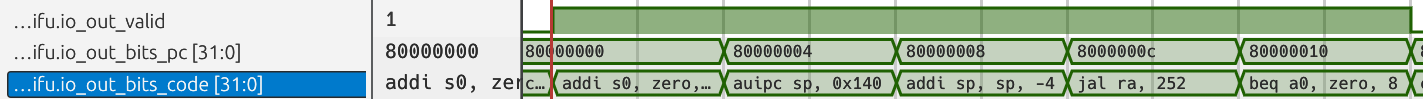
\includegraphics[width=1\linewidth]{imaged.png}\\[0.5em]
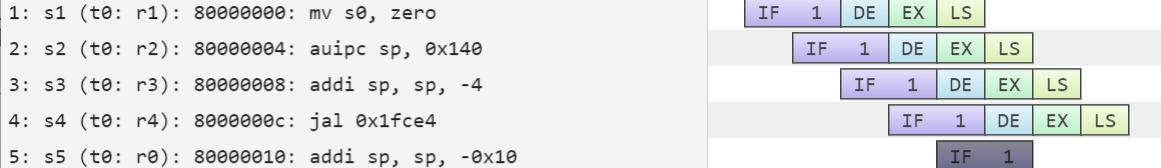
\includegraphics[width=1\linewidth]{imagee.png}
\caption{BRAM 一周期延迟隐藏的取指}
\end{figure}

控制流预测部分则采用了简单利于时序的静态方案。当前分支目标缓存仅保留
8 项 BTB 表项，并配合 BTFN 策略使用：当 BTB 命中后，只有 JAL
或向后分支会被预测为 taken，其中``向后''直接由分支立即数的符号位表示，在 EXU 中检测到分支时更新
，而不额外引入更复杂的历史状态。
后端校验时也\textbf{不需要条件分支比较完整预测目标与真实目标，只需要检查预测方向是否一致}；
因为对条件分支而言，方向一旦判断错误就必然需要重定向，而方向正确时目标地址已由
\texttt{PC+imm} 唯一确定。这样既减少了比较逻辑，也避免把无必要的目标比对放进关键路径。

\begin{table}[htbp]
\centering
\caption{不同 BTB 表项数下的预测命中率对比}
\scriptsize
\begin{tabular}{ccccccc}
\toprule
\textbf{BTB 表项数} & 2 & 4 & 8 & 16 & 32 & 64 \\
\midrule
\textbf{预测准确率} & 33.89\% & 48.64\% & 63.02\% & 65.86\% & 66.53\% & 66.64\% \\
\bottomrule
\end{tabular}
\end{table}

从仿真数据看，BTB 表项数从 2 项增加到 4 项时，命中率提升
14.75 个百分点；从 4 项增加到 8 项时，继续提升 14.38
个百分点，说明较小 BTB 容量下冲突缺失仍然是前端控制流预测的主要损失来源。
但当表项数超过 8 项后，收益迅速收敛：16 项相比 8 项只提升
2.84 个百分点，32 项相比 16 项只提升 0.67 个百分点，64
项相比 32 项仅提升 0.11 个百分点。也就是说，在当前测试负载下，
8 项 BTB 已经覆盖了大部分高频跳转目标，继续增大表项数主要只能减少少量低频冲突。

因此最终实现选择 8 项 BTB 作为面积、时序和性能之间的折中。
更大的 BTB 会增加索引、标记比较和目标选择路径上的寄存器与组合逻辑规模，
对时序收敛不利；而 8 项配置与 64
项配置的命中率差距仅为 3.62 个百分点，性能收益不足以抵消额外时序压力。

\subsection{译码级前移与阻塞削减}

为了减轻 EXU 的组合深度，IDU
并不只负责翻译 opcode，而是在译码阶段就完成一部分后续高频使用的预计算。首先，指令格式和类型在
IDU 中以\textbf{独热码}形式生成，后续各级只需按位判断是否属于 load、store、branch、jal
等类别，不必重复构造一组完整译码条件。其次，\texttt{PC+imm}、\texttt{rs1+imm}
等\textbf{结果也在 IDU 中提前形成}，其中前者直接服务于分支和 JAL
目标地址，后者直接服务于 load/store/JALR 的地址生成。这样可以把最常用的加法运算从
EXU 中拆出去，\textbf{缩短 EXU 上的组合链路}。

IDU 还提前完成了两类会显著影响后端关键路径的工作。其一是 CSR
读取：当前指令需要访问的 CSR 在译码阶段就发起单读端口访问，并把读出值直接作为
EXU 输入，\textbf{避免在 EXU 中再使用 CSR 读后 Mux 路径}。其二是异常与返回类控制流的下一跳选择：\texttt{ecall}
对应的 \texttt{mtvec}、\texttt{mret} 对应的 \textbf{\texttt{mepc}
在 IDU 中预先选成静态下一跳，减轻 EXU
控制流选择压力}。与此同时，对于本来就不需要第二源寄存器的指令，IDU 会直接把
\texttt{rs2} 置为 0，使旁路网络\textbf{不对无效的 \texttt{rs2}
地址进行冲突匹配}，从而减少不必要的阻塞与停顿判定。

\subsection{执行与访存关键路径压缩}

执行级的核心优化是尽可能提早发起访存，同时把不必要留在关键路径上的整理逻辑移走。对
load/store 指令，EXU 直接使用 IDU 已经算好的 \texttt{rs1+imm}
作为目标地址，并在本级构造访存请求；这样在底层存储器是一周期返回时，下一拍 LSU
即可接到响应数据。对于 store，字节写、半字写的掩码生成以及写数据对齐都\textbf{通过
Mux 组合网络完成，而不是使用变量位移指令}实现。这样做虽然在功能上等价，但综合后通常能得到更可控的硬件结构，
\textbf{避免将可变移位器引入访存通路}。

与之对应，LSU 的职责被刻意压缩为``传递原始结果与元信息''，而不是在本级完成全部
load 数据整理。当前设计把地址低位、\texttt{func3} 和原始 32 位读数据一并传给
WBU，再由 WBU 完成字节/半字抽取以及符号扩展、零扩展。这样安排的原因是：在板级实现中，\textbf{BRAM
输出到 LSU 的布线已经较长}，如果在 LSU
立刻叠加位扩展和结果选择逻辑，会进一步压缩时序余量。把这些工作后\textbf{移到 WBU
后，LSU 关键路径更短}，而写回级本身又具备更充足的组合预算，整体上更有利于频率与布线收敛。

虽然会导致旁路网络在 load-use 情况下的停顿多一拍，但评估认为频率提升带来的 IPC 增加可以弥补这一点。

\section{RV32I CPU的特色功能设计}

本章重点说明 CPU 内核自身在基础 RV32I 指令之外补充实现的功能。这些功能一方面用于支撑更完整的软件运行环境，
另一方面也使 CPUCore 能够在不同 SoC 封装中复用。

\subsection{CSR 与机器模式控制流支持}

CPU 内核实现了面向机器模式运行环境的 CSR 子集，支持
\texttt{mstatus}、\texttt{mtvec}、\texttt{mepc}、\texttt{mcause}、
\texttt{mcycle}、\texttt{mcycleh}、\texttt{mvendorid} 和 \texttt{marchid}
等寄存器，并实现了 \texttt{CSRRW}、\texttt{CSRRS}、\texttt{ECALL} 与
\texttt{MRET} 相关路径。该部分不是完整的 RISC-V 特权级实现，但已经覆盖了启动
RT-Thread 所需的基本机器模式控制流。

CSR 访问被拆分到流水线中处理：IDU 在译码阶段根据指令高 12 位发起 CSR
读取，并提前选择 \texttt{ecall} 对应的 \texttt{mtvec} 或 \texttt{mret}
对应的 \texttt{mepc} 作为静态跳转目标；EXU 再根据指令类型生成 CSR
写回使能、写地址和写数据；WBU 在最终提交点统一更新 CSR 文件。这样既保持了顺序提交语义，也避免在
EXU 中再叠加较长的 CSR 读后选择路径。

\subsection{可桥接 AXI4 的存储访问接口}

CPUCore 内部的取指和访存接口使用两路 SimpleBus：IFU 负责指令读取，LSU/数据访存通路负责
load/store 请求。为了让 CPU 内核能够接入更通用的 SoC 总线，工程中实现了
\texttt{DualSimpleBusToAXI4} 桥接模块，将 IFU 与 LSU 两路 SimpleBus
请求汇聚为一路 AXI4 master 接口。

该桥接模块在空闲状态下优先接受 LSU 请求，避免数据访存长期被取指流阻塞；读请求通过
AXI4 \texttt{AR/R} 通道完成，写请求通过 \texttt{AW/W/B} 通道完成，并用状态机记录
\texttt{AW} 与 \texttt{W} 两个通道是否已经握手。当前竞业达 JYD FPGA 顶层为了适配板级
IROM、DRAM 和外设桥，没有启用 AXI4 版本的顶层接口；但 CPU 顶层和桥接模块已经保留，
便于后续切换到 AXI4 内存、AXI4 交叉开关或其他 SoC 验证环境。

\newpage

\section{设计总结}

本项目完成了从 CPU 微结构、存储系统、板级外设映射到上板验证的完整设计。
最终 CPU 内核支持 RV32I 全部 37 条整数指令，并补充实现了 \texttt{CSRRW}、
\texttt{CSRRS}、\texttt{ECALL}、\texttt{MRET} 以及若干机器模式 CSR，
能够支撑赛题测试程序和更完整的软件运行环境。
将指令执行、流水线控制、访存接口、异常返回和 FPGA 顶层适配整合成了可以稳定运行的系统。

从架构上看，CPU 采用 IFU--IDU--EXU--LSU--WBU 五级顺序单发射流水线。
流水线内部实现了寄存器旁路、load-use 停顿、分支预测错误冲刷等控制机制；
前端使用 8 项 BTB 配合 BTFN 静态预测，在较小硬件开销下覆盖主要控制流热点；
后端则将地址生成、CSR 读取、跳转目标预选等逻辑适当前移到 IDU，
并把 load 数据整理后移到 WBU，以降低 EXU/LSU 关键路径压力。
这些取舍在不显著增加面积和设计复杂度的前提下，提高了 FPGA 上的时序收敛能力和有效吞吐率。

性能方面，本设计在 Vivado 2024.2 下完成综合与实现，CPU 核心工作频率达到
\textbf{250 MHz}，且 250 MHz 约束下 WNS 为正、无时序违例。
在竞业达数字孪生平台上，src0、src1、src2、test\_src 四组程序均完成上板验证；
其中三组性能测试运行时间分别为 \textbf{8.7 s}、\textbf{9.8 s} 和
\textbf{10.6 s}，平均 \textbf{CPI 为 1.61}，对应 \textbf{IPC 为 0.62}。
这些数据说明，虽然项目仍是顺序单发射流水线，但通过 BRAM 化存储器、连续取指、
轻量级分支预测和关键路径拆分，已经在功能正确性、频率和流水线利用率之间取得了较好的平衡。

CPUCore 还保留了可桥接 AXI4 的存储访问接口，便于后续接入更通用的 SoC 验证环境。
本作品既满足初赛要求，也具备继续扩展到更复杂存储层次、更强分支预测或更完整特权级支持的基础。

总体而言，本项目展示了一条面向 FPGA 落地的 RISC-V CPU 设计路线：
先保证 RV32I 指令和板级运行正确，再围绕真实时序瓶颈进行流水线与存储系统优化，
最后用上板运行时间、CPI、IPC 和频率数据量化设计效果。

\newpage
\appendix
\section{附录}

\subsection{代码清单}

以下代码清单选取生成后 Verilog 中的核心逻辑，并对无关端口、调试信号和重复连线进行了删节，以便展示关键设计思想。

\begin{lstlisting}[style=svcode,caption={CPUCore.sv / CPUCore：预测错误后的重定向与流水线冲刷}]
wire redirectNow = _exu_io_out_valid & _exu_io_predWrong;
wire redirectPendingFire = _ifu_io_pc_ready & redirectPendingReg;

always @(posedge clock) begin
  if (reset) begin
    redirectPendingReg <= 1'h0;
    pc <= resetPC;
    validReg_3 <= 1'h0;  // IFU -> IDU
    validReg_4 <= 1'h0;  // IDU -> EXU
    validReg_5 <= 1'h0;  // EXU -> LSU
    validReg_6 <= 1'h0;  // LSU -> WBU
  end
  else begin
    redirectPendingReg <= redirectNow
      | (~redirectPendingFire & redirectPendingReg);

    if (_ifu_io_pc_ready)
      pc <= redirectNow ? _exu_io_nxtPC
        : redirectPendingFire | ~redirectPendingReg
            ? nxtPredictedPC
            : redirectTargetReg;

    validReg_3 <= allowIn_3
      ? _ifu_io_out_valid & ~activeRedirectValid
      : ~activeRedirectValid & validReg_3;
    validReg_4 <= allowIn_4
      ? _idu_io_out_valid & ~redirectNow
      : ~redirectNow & validReg_4;
  end

  if (redirectNow)
    redirectTargetReg <= _exu_io_nxtPC;
end
\end{lstlisting}

\begin{lstlisting}[style=svcode,caption={IDU.sv / IDU：CSR 读取与静态跳转目标预选}]
assign io_csrRead_en = io_in_valid;
assign io_csrRead_addr = io_in_bits_code[31:20];

assign io_out_bits_info_csrReadData = io_csrRead_data;
assign io_out_bits_info_staticNextPCOrCSRTarget =
  io_out_bits_info_isECall_0
    ? io_csrJmpTarget_mtvec
    : io_out_bits_info_isMRet_0
        ? io_csrJmpTarget_mepc
        : io_in_bits_pc + 32'h4;

assign io_out_bits_info_pcAddImm = io_in_bits_pc
  + io_out_bits_info_imm_0;
assign io_out_bits_info_reg1AddImm = _bypassMux_io_outData1
  + {{21{io_in_bits_code[31]}}, io_in_bits_code[30:20]};
\end{lstlisting}

\begin{lstlisting}[style=svcode,caption={EXU.sv / EXU：跳转判定、预测错误与 CSR 写回}]
wire isCSRRW = io_in_bits_code[14:12] == 3'h1
  & io_in_bits_info_typ[8];
wire dbgIsCSRJmp = io_in_bits_info_isECall
  | io_in_bits_info_isMRet;

assign io_jmpHappen =
  (dbgIsBranch & takeBranch) | dbgIsJALR | dbgIsJAL | dbgIsCSRJmp;
assign io_predWrong =
  dbgIsJALR | dbgIsCSRJmp
  | (isBranch & (takeBranch ^ io_in_bits_pred_take))
  | (dbgIsJAL & ~io_in_bits_pred_hit);

assign io_nxtPC =
  dbgIsJALR ? {io_in_bits_info_reg1AddImm[31:1], 1'h0}
  : (dbgIsJAL | isTakenBranch) ? io_in_bits_info_pcAddImm
  : io_in_bits_info_staticNextPCOrCSRTarget;

assign io_out_bits_exuWriteBack_csr_en =
  isCSRRW | (isCSRRS & (|io_in_bits_info_reg1));
assign io_out_bits_exuWriteBack_csr_addr =
  io_in_bits_info_isECall ? 12'h341 : io_in_bits_code[31:20];
assign io_out_bits_exuWriteBack_csr_data =
  io_in_bits_info_isECall ? io_in_bits_pc
  : isCSRRW ? io_in_bits_info_reg1
  : io_in_bits_info_csrReadData | io_in_bits_info_reg1;
\end{lstlisting}

\begin{lstlisting}[style=svcode,caption={DualSimpleBusToAXI4.sv / DualSimpleBusToAXI4：双 SimpleBus 到 AXI4 的桥接}]
reg [2:0] state;
reg       selLSU;
reg [31:0] reqAddr, reqWData;
reg [2:0]  reqSize;
reg [3:0]  reqWMask;
reg        awSent, wSent;

wire hasReq = io_lsu_req_valid | io_ifu_req_valid;
wire takeLSU = io_lsu_req_valid;

assign io_lsu_req_ready = state == 3'h0;
assign io_ifu_req_ready = (state == 3'h0) & ~takeLSU;

always @(posedge clock) begin
  if (reset)
    state <= 3'h0;
  else begin
    casez (state)
      3'h0: state <= hasReq ? (takeLSU && io_lsu_wen ? 3'h3 : 3'h1) : 3'h0;
      3'h1: state <= io_out_arready ? 3'h2 : 3'h1;
      3'h2: state <= io_out_rvalid  ? 3'h0 : 3'h2;
      3'h3: state <= (awSent | io_out_awready) & (wSent | io_out_wready)
                      ? 3'h4 : 3'h3;
      3'h4: state <= io_out_bvalid  ? 3'h0 : 3'h4;
    endcase
  end
end

assign io_out_arvalid = state == 3'h1;
assign io_out_rready  = state == 3'h2;
assign io_out_awvalid = (state == 3'h3) & ~awSent;
assign io_out_wvalid  = (state == 3'h3) & ~wSent;
assign io_out_bready  = state == 3'h4;
\end{lstlisting}

\begin{lstlisting}[style=svcode,caption={CPUTop.sv / CPUTop：CPUCore 接入 AXI4 桥接模块}]
CPUCore core (
  .io_irom_req_ready  (_memBridge_io_ifu_req_ready),
  .io_irom_req_valid  (_core_io_irom_req_valid),
  .io_irom_addr       (_core_io_irom_addr),
  .io_irom_resp_valid (_memBridge_io_ifu_resp_valid),
  .io_irom_rdata      (_memBridge_io_ifu_rdata),
  .io_dram_req_ready  (_memBridge_io_lsu_req_ready),
  .io_dram_req_valid  (_core_io_dram_req_valid),
  .io_dram_addr       (_core_io_dram_addr),
  .io_dram_wdata      (_core_io_dram_wdata),
  .io_dram_wmask      (_core_io_dram_wmask),
  .io_dram_wen        (_core_io_dram_wen)
);

DualSimpleBusToAXI4 memBridge (
  .io_ifu_req_valid (_core_io_irom_req_valid),
  .io_ifu_addr      (_core_io_irom_addr),
  .io_lsu_req_valid (_core_io_dram_req_valid),
  .io_lsu_addr      (_core_io_dram_addr),
  .io_lsu_wdata     (_core_io_dram_wdata),
  .io_lsu_wmask     (_core_io_dram_wmask),
  .io_lsu_wen       (_core_io_dram_wen),
  .io_out_awvalid   (io_master_awvalid),
  .io_out_awaddr    (io_master_awaddr),
  .io_out_wvalid    (io_master_wvalid),
  .io_out_wdata     (io_master_wdata),
  .io_out_arvalid   (io_master_arvalid),
  .io_out_araddr    (io_master_araddr),
  .io_out_rready    (io_master_rready)
);
\end{lstlisting}

\subsection{工程目录结构}

\makeatletter
\newcommand{\mydotfill}{%
  \leavevmode
  \leaders\hbox to 1em{%
    \hss
    \raisebox{0.3ex}{\textcolor{gray}{.}}%
    \hss
  }\hfill\kern0pt
}
\makeatother

\begin{minipage}{0.9\textwidth}
\centering
\dirtree{%
.1 jyd/ \mydotfill 工程根目录.
.2 npc/ \mydotfill CPU 设计、SoC 封装与仿真工程.
.3 design/src/ \mydotfill Chisel 源码：流水线、总线、外设桥.
.3 build/gened/verilog/ \mydotfill 生成后的 Verilog/SystemVerilog.
.3 sim/ \mydotfill Verilator 仿真与性能统计.
.3 scripts/ \mydotfill 辅助脚本.
.2 jyd-tests/ \mydotfill 竞业达样例程序与 COE 处理脚本.
.2 abstract-machine/ \mydotfill bare-metal 运行环境与平台抽象.
.2 nemu/ \mydotfill RISC-V 参考执行环境.
.2 .github/workflows/ \mydotfill 自动化回归流程.
}
\end{minipage}

\newpage

\subsection{参考资料}

\begin{enumerate}[label={[\arabic*]},leftmargin=3em]
\item 全国大学生集成电路创新创业大赛组委会. 第十届集创赛初赛作品提交要求.
\item 竞业达企业命题组. ``竞业达''企业命题作品材料参考模板.
\item 竞业达企业命题组. FPGA 开发板远程连接操作手册, 2026.
\item 竞业达企业命题组. 上板实验说明与赛题测试程序资料.
\item RISC-V International. The RISC-V Instruction Set Manual, Volume I: Unprivileged ISA.
\item RISC-V International. The RISC-V Instruction Set Manual, Volume II: Privileged Architecture.
\end{enumerate}

\subsection{AI工具使用声明}

工具名称：ChatGPT 5.3/5.4。

使用场景与用途如下：

\begin{itemize}
\item 工具脚本编写：自动插入注释、自动修改宏名、将 coe 文件转 bin 并反编译成汇编、自动打包代码、自动移除 dpi 调用、自动替换 Vivado 工程文件为新 Verilog 代码。
\item 部分功能的实现或重构：根据团队的优化思路快速形成初版改动。
\item 仿真代码的部分重构：使用 AI 重构流水线日志的生成方式。
\item 分析时序报告：辅助解读 Vivado 的时序报告。
\item 辅助撰写技术文档：润色文字表达，辅助图表绘制。
\end{itemize}

AI 生成内容占比估计（文字/代码/设计）：

\begin{itemize}
\item 文字：15\%
\item 代码：10\%
\item 设计：5\%
\end{itemize}
\end{document}
